\chapter{Introduction au Big Data} \label{chap:big-data-intro}
	\section{Introduction}
		Big Data est un terme associé aux données massives, rapidement générées, ayant une grande diversité que les  outils traditionnels sont incapables de gérer ces données. En Big Data,  tout type de données peut être utilisé, et ce en vue de livrer la bonne information à la bonne personne et au bon moment dans le but d'aider à prendre les bonnes décisions. Dans ce chapitre, nous  présentons brièvement un des processus d'analyse de données. Ensuite, nous décrivons quelques concepts impliqués dans un processus d'analyse des données massives. Enfin, nous parcourons un ensemble de technologies utilisées dans l'analyse des données à grande échelle.
			
	\section{Processus d'analyse de données massives}
	%668
Les étapes d'un processus d'analyse de données, à grande échelle ou non, sont différentes selon le processus adopté.  Ce dernier peut impliquer plusieurs besoins et concepts. En particulier, on note le besoin du stockage de données massives, du traitement de données massives et le besoin de la visualisation des résultats des traitements appliqués. Le choix du traitement à appliquer sur les données est dirigé par les objectifs de  l'analyse menée. Par exemple, une analyse peut envisager la création d'un système de recommandations dans les sites Internet, la conception d'un outil de prédiction basé sur les données historiées, un système de suivi en temps réel, etc.  Ces applications appuient sur des algorithmes basés sur les mathématiques, en particulier les mathématiques statistiques et probabilistes. Afin d'assurer l'efficacité de l'analyse de données massives, la coopération de plusieurs ressources accélère considérablement les étapes de l'analyse, c'est ce que l'informatique distribuée a apporté.
\paragraph{Exemple d'un  processus d'analyse de données} \label{sec:process-data-analysis}~

Le processus d'analyse de données passe généralement par des étapes classiques. A ces étapes peuvent s'ajouter d'autres étapes intermédiaires ou supplémentaires. 
Pour précision, non seulement  ces étapes peuvent s'appliquer dans le cas  où les données sont volumineuses,  mais aussi dans le cas des données en provenance des outils traditionnels comme les bases de données relationnelles. IBM Knowledge Center \footnote{Source : \url{https://www.ibm.com/support/knowledgecenter/fr/SSEPGG_9.5.0/com.ibm.im.easy.doc/c_dm_process.html}, consultée le $06/08/2018$.} a résumé le processus de l'analyse de données dans les étapes suivantes :
définition de problème, exploration de données, préparation de données, modélisation, évaluation et enfin l'étape de déploiement.


\textbf{Définition de problème} C'est le point d'entrée vers tout projet d'analyse de données. Les objectifs doivent être clairs. A la fin de cette étape, on connait les objectifs de l'analyse, mais pas forcément comment cette analyse va être menée en terme de technologies utilisées,  les méthodes statistiques, etc. \par

\textbf{Exploration de données } Ce que caractérise cette étape, c'est la découverte de la nature  des données, les sources des données, la qualité des données, etc. \par

\textbf{Préparation de données} \label{par:step-preparedata} C'est durant cette phase que se passent les opérations d'ETL (Extract-Transform-Load), ce sont les opérations de transformation, de nettoyage et de chargement des données vers les entrepôts de données (voir ETL dans la section \ref{sec:etl}). Durant cette étape,  ce ne sont que  des tentatives  faites pour créer le schéma de données.  Dans certains cas, cela amène  à chercher des sources complémentaires de données ou bien à appliquer de nouvelles transformations  sur les données. \par
%Tel qu'un  schéma comporte les différentes tables, les attributs pertinents et autres. 

\textbf{Modélisation} A l'issue de cette étape, un modèle de qualité est créé. Ce modèle  doit  répondre aux objectifs précédemment établis dans l'étape de la définition du problème. Cette étape implique des principes en statistiques, probabilités, \textit{machine learning}, etc. \par

\textbf{Evaluation} C'est à cette étape qu'on valide le modèle créé à l'étape de  Modélisation. L'évaluation et la validation du modèle prennent en compte les objectifs prédéfinis; si le modèle répond aux attentes précédemment exprimées. \par

\textbf{Déploiement}  C'est l'utilisation  des outils existants ou  la mise en place d'une solution permettant d'exploiter les résultats obtenus lors de l'application du modèle créé sur les données disponibles. Par exemple, la  visualisation des résultats de l'analyse  sous forme d'un tableau d'indicateurs sur une page Web. \par
\section{Quelques concepts associés au Big Data}
Etant donné que le domaine du Big Data implique plusieurs concepts, nous présentons une liste de concepts  non exhaustive. 
\subsection{Définition du Big Data : Volume, Vélocité, Variété et Véracité}
		IBM définit le Big Data suivant les quatre dimensions suivants : volume, variété, vélocité et véracité. 
		\paragraph{Volume de données}~
		La quantité de données manipulées par les outils traditionnels de la gestion des données est de l'ordre de gigaoctets (GO) et de téraoctets (TO). Toutefois, le Big Data est mesuré en pétaoctets (PO), exaoctets (EO), voire plus. Une des premières applications du Big Data est la recherche dans Word-Wide Web (WWW). Selon l'étude (\cite{6567202}, $2013$) de l'International Data Corporation (IDC), le volume de données  va atteindre $40$ zettaoctets\footnote{ $ 1$ ZO = $1,000,000,000,000$ GO. } par  entreprise en $2020$. Dans un rapport récent (\cite{IDC-data}, $ 2018 $), 
		IDC prédit que le volume de la  datasphère  planétaire, c'est-à-dire le volume de nouvelles données créées et répliquées chaque année, appelée  Global Datasphere en anglais,  passera de $  33 $ ZO en $2018$ à $175$ ZO d'ici $ 2025 $.
		
		\paragraph{Vélocité de données} ~
		le Big Data est généré par des milliards
		d'appareils. Les données générées sont communiquées avec la vitesse de la lumière via l'Internet. L'augmentation de la vitesse de l'Internet est une  des raisons ayant contribué à l'augmentation de la vitesse de la génération de données.	
		%la vitesse décrit la fréquence de la génération et du partage des données. Autrement dit, les données sont générées rapidement et doivent être traitées rapidement pour extraire les informations  pertinentes.
		Par exemple, Wallmart (international discount retail chain) génère environ   $2.5$ pétaoctets de données chaque  heure via les transactions de ses consommateurs\footnote{Source : \url{https://www.bernardmarr.com/default.asp?contentID=690}, consultée le $ 30/06/2018 $.}.
		\paragraph{Variété de données} \label{variete-data}
		
		Le Big Data inclut toutes les formes de données, des fonctions diversifiés des données et des sources variées des données.
		
		Le premier aspect de la variété  des données massives est la \textbf{forme} de celles-ci. Les données manipulées incluent du texte, des graphes, des cartes, des vidéos, des photos, etc.
		
		Le deuxième aspect de la variété des données massives concerne les \textbf{fonctions} assurées par ces données. Des données sont issues des conversations humaines, d'autres des transactions des consommateurs, ou bien des données archivées, etc.
		
		Les \textbf{sources} du Big Data est le troisième aspect de  variété. Des données sont en provenance des téléphones mobiles, des tablettes ou des ordinateurs portables, des fichiers journaux, des réseaux de capteurs, etc. Les sources du Big Data peuvent être classées en trois grandes catégories : communications \textbf{\textit{human to human}} comme les conversations échangées dans les réseaux sociaux, communications \textbf{\textit{ human to machine}} comme l'accès des utilisateurs aux données dans le Web et enfin communications \textbf{\textit{machine to machine}} comme les données issues de la communication entre les capteurs dans un réseau de capteurs.
		%au-delà des données des transactions habituelles des consommateurs, les données manipulées sont en provenance de sources différentes et de formats différents. Par exemple: des vidéos, des documents, des commentaires, des données géospatiales, des journaux, etc. Les grands ensembles de données sont constitués de données structurées et non structurées, publiques ou privées, locales ou distantes, partagées ou confidentielles, complètes ou incomplètes, etc.
		\paragraph{Véracité de données}
		
		La véracité concerne la crédibilité et la qualité de données. La mauvaise qualité de données est due à de nombreuses raisons, telles que les pannes techniques comme le dysfonctionnement des appareils comme les capteurs, les erreurs humaines,  etc. De plus, les données peuvent être intentionnellement erronées pour des raisons de concurrence ou des raisons stratégiques.
	
		\subsection{L'architecture standard du Big Data}
		
		L'architecture standard du Big Data présentée dans ce qui suit est celle proposée dans  \cite{anil-big-data}. Cette architecture  est composée des couches suivantes :  \textit{Data sources}, \textit{Data Ingest}, \textit{Batch processing}, \textit{Stream Processing}, \textit{Data organizing}, \textit{Infrastructure}, \textit{Distributed File System} et enfin la couche \textit{Data consuption}. 
		%Pour  chaque couche, il existe au moins une technologie.
		 La Figure \ref{fig:bigdata-architecture} reprend l'organisation des différentes couches de cette architecture.
		 		\begin{figure}[h]
		 	\captionsetup{justification = centering}
		 	\centering
		 	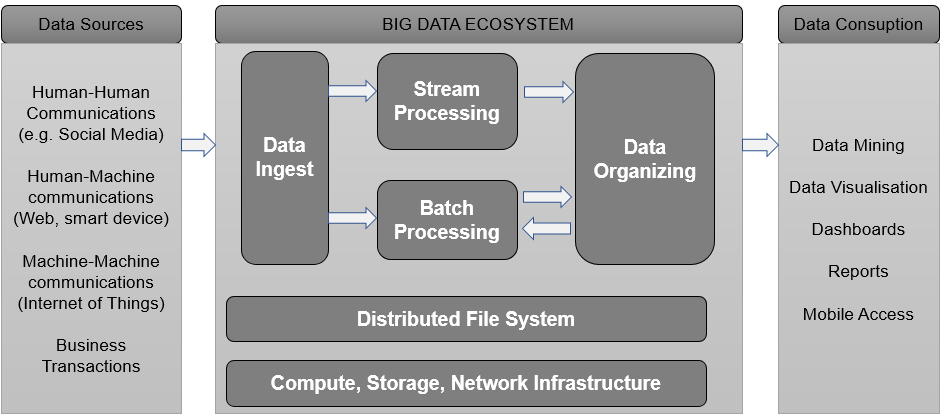
\includegraphics[width=\linewidth]{illustrations/bigdata-architecture}
		 	\caption{Architecture standard du Big Data. Source :  \cite{anil-big-data}}
		 	\label{fig:bigdata-architecture}
		 \end{figure}
		
		Dans un premier temps, les données sont   accueillies   via la couche  \textit{ingest system} par diverses sources de données. Ensuite, les données sont traitées selon deux modes :  \textit{stream processing } et  \textit{batch processing}.  Les résultats de ce traitement peuvent être envoyés vers les bases de données NoSQL (voir la section \ref{sec:nosql}) pour une utilisation ultérieure, ou bien être utilisés  comme entrées pour d'autres applications.  Une solution Big Data comprend typiquement  ces  couches logiques. Chaque  couche peut être représentée par une ou plusieurs technologies disponibles. Reprenons chaque couche logique:
		
		
		%\begin{description}
			\paragraph{Data sources layer} Le choix des sources de donnés pour une application donnée dépend des objectifs qui dirigent l'analyse en question. Les sources avec leurs différents aspects sont détaillées dans la section \ref{variete-data}.
		\paragraph{Data Ingest layer} Cette couche permet de récupérer les données depuis les différentes sources de données. Les données sont accueillies à travers des points d'entrées multiples. Ces points  sont capables de recevoir  ces données ayant une vélocité variable ainsi qu'une quantité aussi variable.  Après avoir traversé  la couche \textit{Data Ingest}, les données sont envoyées au \textit{batch processing system}, au \textit{stream processing system}, ou bien à un système de stockage particulier.
		\paragraph{Batch processing layer} Les données reçues sur cette couche sont celles en provenance du \textit{Data Ingest} ou bien d'une des bases de données NoSQL. Ces données sont ensuite traitées, par exemple, en utilisant les techniques de la programmation parallèle en vue de fournir les résultats souhaités dans un temps raisonnable. La présente couche doit avoir connaissance des sources de données, des types de données, des algorithmes qui vont travailler sur ces données et enfin des résultats souhaités. Les résultats des traitements peuvent être utilisés par une des applications ou bien être sauvegardés dans une des bases de données adaptées.\par
		\paragraph{Stream Processing layer} Cette couche approvisionne les données directement d'une des entrées du \textit{Data Ingest layer}; c'est ce qui différencie cette couche de la couche Batch processing layer. En revanche, \textit{Stream Processing} est similaire à la couche   \textit{Batch processing} en matière  des techniques de la programmation parallèle utilisées ainsi que la nécessité d'avoir les détails sur les sources des données, les types de données et les résultats souhaités.\par
		\paragraph{Data organizing layer} Le rôle de cette couche est d'organiser les données en provenance de la  couche  \textit{Stream Processing} et de la couche \textit{Batch processing}. Cette couche est représentée par les bases de données NoSQL. 
		 %afin de faciliter l'accès à ces dernières. Ce sont les  données obtenues  de la part .
		\paragraph{Infrastructure layer} Cette composante est responsable de la gestion des ressources de stockage, des ressources du calcul et de la gestion de la communication. Les fonctionnalités de cette couche sont typiquement fournies à travers le cloud computing.
		\paragraph{Distributed File System layer} Cette couche permet de stocker une grande quantité de données, de sorte que ces données soient rapidement et facilement accessibles à toutes les couches qui forment un système  Big Data. C'est ce qu'assure, par exemple, Hadoop Distributed File System (HDFS).
		\paragraph{Data consumption layer} Cette dernière couche utilise les résultats obtenus par les couches de l'analyse. Les résultats fournis peuvent être exprimés avec des rapports, des tableaux d'indicateurs, des visualisations, un moteur de recommandation ou tout autre format.
	\subsection{Les bases de données NoSQL (Not Only SQL) } \label{sec:nosql}
	\paragraph{Introduction } ~
	
    Au cours de ces dernières années, on constate une révolution dans le stockage de données non structurées ayant une taille importante.  De plus,  les objets à sauvegarder sont complexes; ils sont issus de sources hétérogènes.  Cette complexité a mis en question les performances des bases de données relationnelles. 
	
	Le terme NoSQL est apparu pour la première fois en $ 1998 $. Carlo Strozzi \cite{CarloStrozziNosql} a parlé des bases de données relationnelles qui n'utilisent pas le SQL comme langage d'interrogation des tables. Des années plus tard, des solutions  open source basées sur ce concept ont vu le jour. 
	
	Les bases de données relationnelles sont conçues pour gérer les données structurées et sont optimisées pour offrir la précision et la cohérence de données. De plus, elles sont utilisées par de nombreuses entreprises pour plusieurs raisons comme   la facilité d'utilisation, la disponibilité de plusieurs produits et développeurs, etc. Ces dernières années, avec l'augmentation exponentielle de la quantité de données générées par certaines entreprises, ces dernières ont constaté l'insuffisance des Systèmes de Gestion de Bases de Données Relationnelles (SGBDR) pour répondre à leurs besoins.
	
    %	\paragraph{ Les besoins auxquels répondent NoSQL}  ~
	Les bases de données NoSQL sont conçues pour gérer des  volumes de données importants. Le flux ainsi que la structure de  ces données sont imprévisibles. C'est pourquoi les bases de données relationnelles ne sont pas convenables. L'idée  des bases de données NoSQL, c'est d'abord assurer la capacité de stocker des données à grande échelle dont la  quantité  évolue rapidement, voire exponentiellement.  En deuxième lieu, les données stockées  doivent être interrogées  avec efficacité. Les données stockées dans  les bases de données NoSQL n'obéissent pas à un modèle prédéfini comme c'est le cas pour les bases de données relationnelles. Cette flexibilité est une des caractéristiques des bases de données NoSQL.
	\paragraph{Types de base de données NoSQL} \label{sec:nosql-database}  ~
	
	Il existe quatre catégories distinctes de bases de données NoSQL. Chaque catégorie répond  à des besoins particuliers. On distingue les bases de données clé-valeur, document, graphe et colonne.
	\subparagraph {Clé-valeur} Une base de données de type clé-valeur repose sur le paradigme clé-valeur; chaque donnée, que ce soit un nombre, du texte ou tout autre type est associé à une clé unique. Cette clé est le seul moyen d'accéder aux données stockées.
	Dans les bases de données NoSQL de type clé-valeur, les enregistrements  n'adhèrent pas à une structure prédéfinie. Par exemple, on peut avoir le premier enregistrement de type entier et le deuxième enregistrement de type texte. Cela assure une forte évolutivité grâce à l'absence d'une structure ou de typage. La Figure \ref{fig:key-value-nosql} montre un exemple de données stockées sous forme de paires clé-valeur.
	\begin{figure}[h]
		\captionsetup{justification=centering}
		\centering
		\resizebox{.4\textwidth}{!}{
			% Graphic for TeX using PGF
% Title: /home/hayat/RipeAtlasTraceroutesAnalysis/2019/Rapport_Mai/illustrations/key-value-nosql.dia
% Creator: Dia v0.97+git
% CreationDate: Tue May  7 11:51:50 2019
% For: hayat
% \usepackage{tikz}
% The following commands are not supported in PSTricks at present
% We define them conditionally, so when they are implemented,
% this pgf file will use them.
\ifx\du\undefined
  \newlength{\du}
\fi
\setlength{\du}{15\unitlength}
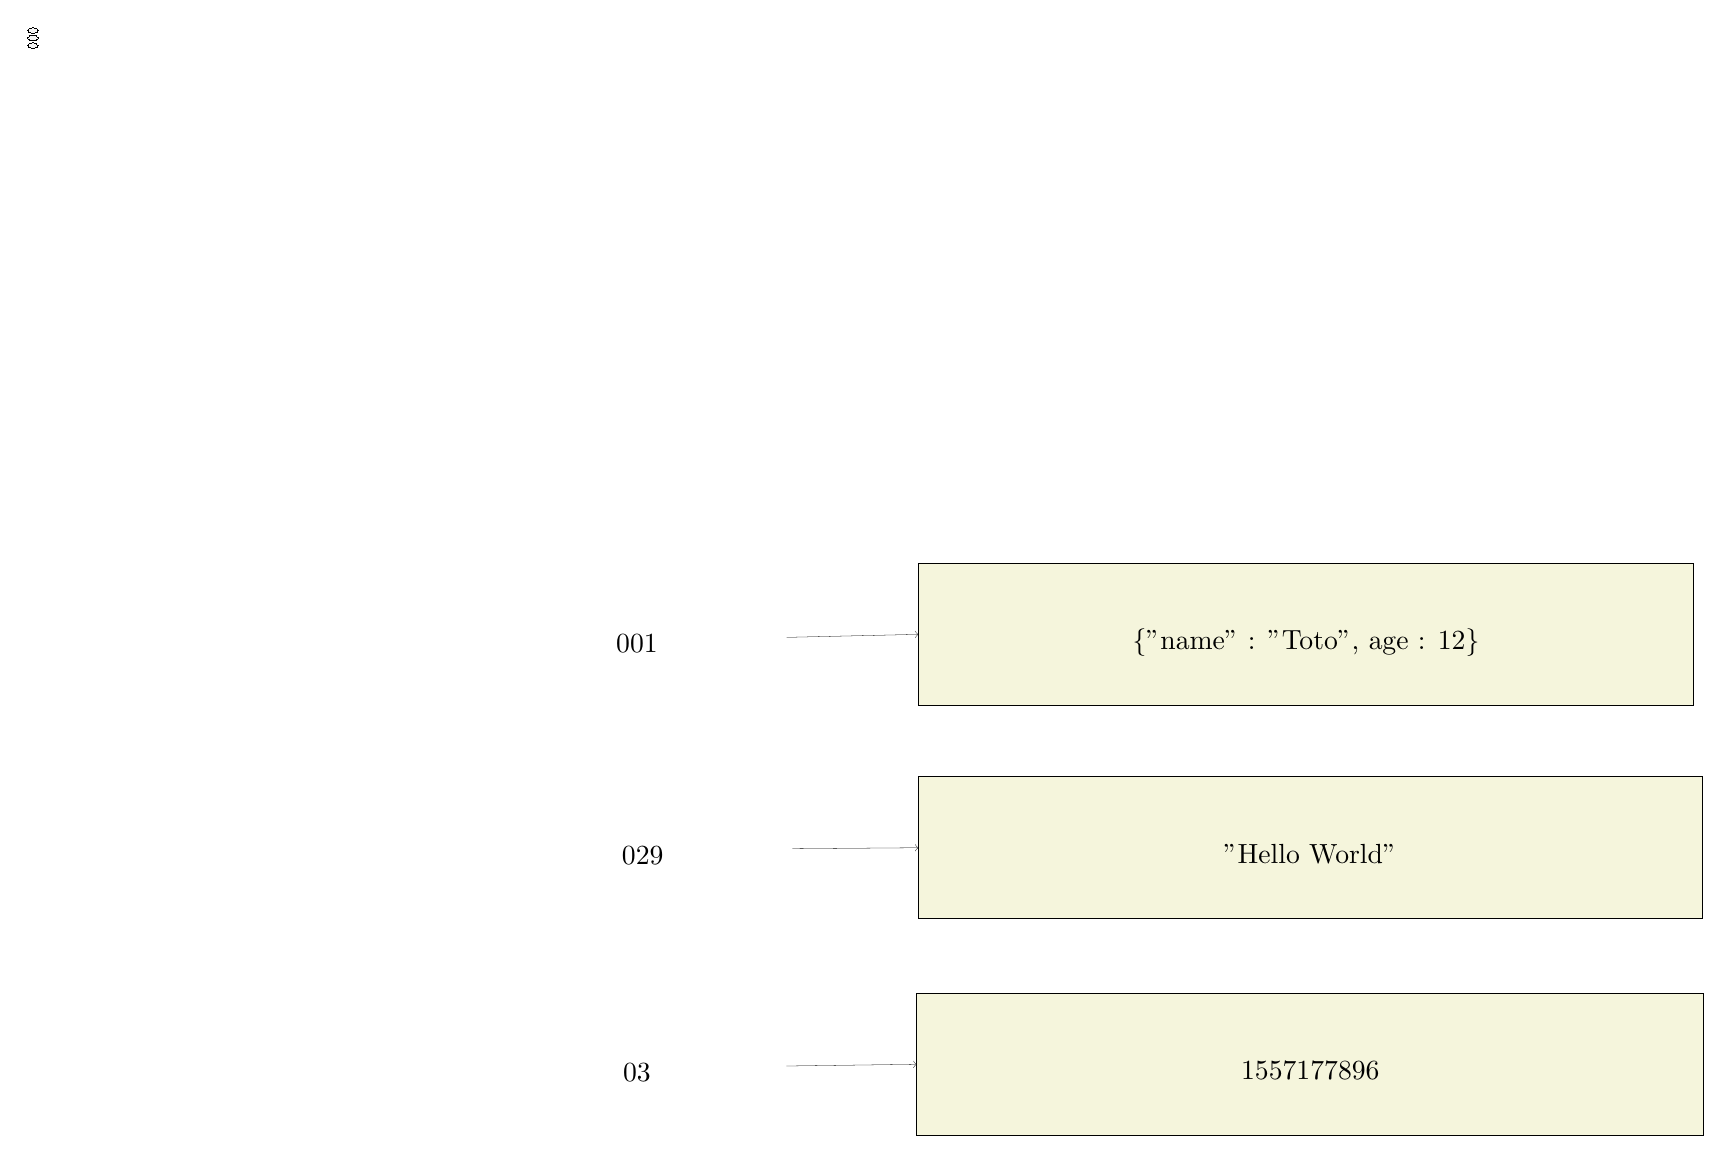
\begin{tikzpicture}[even odd rule]
\pgftransformxscale{1.000000}
\pgftransformyscale{-1.000000}
\definecolor{dialinecolor}{rgb}{0.000000, 0.000000, 0.000000}
\pgfsetstrokecolor{dialinecolor}
\pgfsetstrokeopacity{1.000000}
\definecolor{diafillcolor}{rgb}{1.000000, 1.000000, 1.000000}
\pgfsetfillcolor{diafillcolor}
\pgfsetfillopacity{1.000000}
\pgfsetlinewidth{0.000000\du}
\pgfsetdash{}{0pt}
\pgfsetmiterjoin
\definecolor{diafillcolor}{rgb}{0.960784, 0.960784, 0.960784}
\pgfsetfillcolor{diafillcolor}
\pgfsetfillopacity{1.000000}
\pgfpathellipse{\pgfpoint{7.950991\du}{7.987995\du}}{\pgfpoint{1.899011\du}{0\du}}{\pgfpoint{0\du}{1.012005\du}}
\pgfusepath{fill}
\definecolor{dialinecolor}{rgb}{0.000000, 0.000000, 0.000000}
\pgfsetstrokecolor{dialinecolor}
\pgfsetstrokeopacity{1.000000}
\pgfpathellipse{\pgfpoint{7.950991\du}{7.987995\du}}{\pgfpoint{1.899011\du}{0\du}}{\pgfpoint{0\du}{1.012005\du}}
\pgfusepath{stroke}
% setfont left to latex
\definecolor{dialinecolor}{rgb}{0.000000, 0.000000, 0.000000}
\pgfsetstrokecolor{dialinecolor}
\pgfsetstrokeopacity{1.000000}
\definecolor{diafillcolor}{rgb}{0.000000, 0.000000, 0.000000}
\pgfsetfillcolor{diafillcolor}
\pgfsetfillopacity{1.000000}
\node[anchor=base,inner sep=0pt, outer sep=0pt,color=dialinecolor] at (7.950991\du,8.182995\du){001};
\pgfsetlinewidth{0.000000\du}
\pgfsetdash{}{0pt}
\pgfsetmiterjoin
\definecolor{diafillcolor}{rgb}{0.960784, 0.960784, 0.960784}
\pgfsetfillcolor{diafillcolor}
\pgfsetfillopacity{1.000000}
\pgfpathellipse{\pgfpoint{8.024011\du}{10.672005\du}}{\pgfpoint{1.899011\du}{0\du}}{\pgfpoint{0\du}{1.012005\du}}
\pgfusepath{fill}
\definecolor{dialinecolor}{rgb}{0.000000, 0.000000, 0.000000}
\pgfsetstrokecolor{dialinecolor}
\pgfsetstrokeopacity{1.000000}
\pgfpathellipse{\pgfpoint{8.024011\du}{10.672005\du}}{\pgfpoint{1.899011\du}{0\du}}{\pgfpoint{0\du}{1.012005\du}}
\pgfusepath{stroke}
% setfont left to latex
\definecolor{dialinecolor}{rgb}{0.000000, 0.000000, 0.000000}
\pgfsetstrokecolor{dialinecolor}
\pgfsetstrokeopacity{1.000000}
\definecolor{diafillcolor}{rgb}{0.000000, 0.000000, 0.000000}
\pgfsetfillcolor{diafillcolor}
\pgfsetfillopacity{1.000000}
\node[anchor=base,inner sep=0pt, outer sep=0pt,color=dialinecolor] at (8.024011\du,10.867005\du){029};
\pgfsetlinewidth{0.000000\du}
\pgfsetdash{}{0pt}
\pgfsetmiterjoin
\definecolor{diafillcolor}{rgb}{0.960784, 0.960784, 0.960784}
\pgfsetfillcolor{diafillcolor}
\pgfsetfillopacity{1.000000}
\pgfpathellipse{\pgfpoint{7.949011\du}{13.432005\du}}{\pgfpoint{1.899011\du}{0\du}}{\pgfpoint{0\du}{1.012005\du}}
\pgfusepath{fill}
\definecolor{dialinecolor}{rgb}{0.000000, 0.000000, 0.000000}
\pgfsetstrokecolor{dialinecolor}
\pgfsetstrokeopacity{1.000000}
\pgfpathellipse{\pgfpoint{7.949011\du}{13.432005\du}}{\pgfpoint{1.899011\du}{0\du}}{\pgfpoint{0\du}{1.012005\du}}
\pgfusepath{stroke}
% setfont left to latex
\definecolor{dialinecolor}{rgb}{0.000000, 0.000000, 0.000000}
\pgfsetstrokecolor{dialinecolor}
\pgfsetstrokeopacity{1.000000}
\definecolor{diafillcolor}{rgb}{0.000000, 0.000000, 0.000000}
\pgfsetfillcolor{diafillcolor}
\pgfsetfillopacity{1.000000}
\node[anchor=base,inner sep=0pt, outer sep=0pt,color=dialinecolor] at (7.949011\du,13.627005\du){03};
\pgfsetlinewidth{0.000000\du}
\pgfsetdash{}{0pt}
\pgfsetmiterjoin
{\pgfsetcornersarced{\pgfpoint{0.000000\du}{0.000000\du}}\definecolor{diafillcolor}{rgb}{0.960784, 0.960784, 0.862745}
\pgfsetfillcolor{diafillcolor}
\pgfsetfillopacity{1.000000}
\fill (11.525300\du,7.050000\du)--(11.525300\du,8.850000\du)--(21.369346\du,8.850000\du)--(21.369346\du,7.050000\du)--cycle;
}{\pgfsetcornersarced{\pgfpoint{0.000000\du}{0.000000\du}}\definecolor{dialinecolor}{rgb}{0.000000, 0.000000, 0.000000}
\pgfsetstrokecolor{dialinecolor}
\pgfsetstrokeopacity{1.000000}
\draw (11.525300\du,7.050000\du)--(11.525300\du,8.850000\du)--(21.369346\du,8.850000\du)--(21.369346\du,7.050000\du)--cycle;
}% setfont left to latex
\definecolor{dialinecolor}{rgb}{0.000000, 0.000000, 0.000000}
\pgfsetstrokecolor{dialinecolor}
\pgfsetstrokeopacity{1.000000}
\definecolor{diafillcolor}{rgb}{0.000000, 0.000000, 0.000000}
\pgfsetfillcolor{diafillcolor}
\pgfsetfillopacity{1.000000}
\node[anchor=base,inner sep=0pt, outer sep=0pt,color=dialinecolor] at (16.447323\du,8.145000\du){\{"name" : "Toto", age : 12\}};
\pgfsetlinewidth{0.000000\du}
\pgfsetdash{}{0pt}
\pgfsetmiterjoin
{\pgfsetcornersarced{\pgfpoint{0.000000\du}{0.000000\du}}\definecolor{diafillcolor}{rgb}{0.960784, 0.960784, 0.862745}
\pgfsetfillcolor{diafillcolor}
\pgfsetfillopacity{1.000000}
\fill (11.525300\du,9.760000\du)--(11.525300\du,11.560000\du)--(21.479549\du,11.560000\du)--(21.479549\du,9.760000\du)--cycle;
}{\pgfsetcornersarced{\pgfpoint{0.000000\du}{0.000000\du}}\definecolor{dialinecolor}{rgb}{0.000000, 0.000000, 0.000000}
\pgfsetstrokecolor{dialinecolor}
\pgfsetstrokeopacity{1.000000}
\draw (11.525300\du,9.760000\du)--(11.525300\du,11.560000\du)--(21.479549\du,11.560000\du)--(21.479549\du,9.760000\du)--cycle;
}% setfont left to latex
\definecolor{dialinecolor}{rgb}{0.000000, 0.000000, 0.000000}
\pgfsetstrokecolor{dialinecolor}
\pgfsetstrokeopacity{1.000000}
\definecolor{diafillcolor}{rgb}{0.000000, 0.000000, 0.000000}
\pgfsetfillcolor{diafillcolor}
\pgfsetfillopacity{1.000000}
\node[anchor=base,inner sep=0pt, outer sep=0pt,color=dialinecolor] at (16.502425\du,10.855000\du){"Hello World"};
\pgfsetlinewidth{0.000000\du}
\pgfsetdash{}{0pt}
\pgfsetmiterjoin
{\pgfsetcornersarced{\pgfpoint{0.000000\du}{0.000000\du}}\definecolor{diafillcolor}{rgb}{0.960784, 0.960784, 0.862745}
\pgfsetfillcolor{diafillcolor}
\pgfsetfillopacity{1.000000}
\fill (11.503500\du,12.510000\du)--(11.503500\du,14.310000\du)--(21.501313\du,14.310000\du)--(21.501313\du,12.510000\du)--cycle;
}{\pgfsetcornersarced{\pgfpoint{0.000000\du}{0.000000\du}}\definecolor{dialinecolor}{rgb}{0.000000, 0.000000, 0.000000}
\pgfsetstrokecolor{dialinecolor}
\pgfsetstrokeopacity{1.000000}
\draw (11.503500\du,12.510000\du)--(11.503500\du,14.310000\du)--(21.501313\du,14.310000\du)--(21.501313\du,12.510000\du)--cycle;
}% setfont left to latex
\definecolor{dialinecolor}{rgb}{0.000000, 0.000000, 0.000000}
\pgfsetstrokecolor{dialinecolor}
\pgfsetstrokeopacity{1.000000}
\definecolor{diafillcolor}{rgb}{0.000000, 0.000000, 0.000000}
\pgfsetfillcolor{diafillcolor}
\pgfsetfillopacity{1.000000}
\node[anchor=base,inner sep=0pt, outer sep=0pt,color=dialinecolor] at (16.502406\du,13.605000\du){1557177896 };
\pgfsetlinewidth{0.100000\du}
\pgfsetdash{}{0pt}
\pgfsetbuttcap
{
\definecolor{diafillcolor}{rgb}{0.000000, 0.000000, 0.000000}
\pgfsetfillcolor{diafillcolor}
\pgfsetfillopacity{1.000000}
% was here!!!
\pgfsetarrowsend{to}
\definecolor{dialinecolor}{rgb}{0.000000, 0.000000, 0.000000}
\pgfsetstrokecolor{dialinecolor}
\pgfsetstrokeopacity{1.000000}
\draw (9.850000\du,7.988000\du)--(11.525300\du,7.950000\du);
}
\pgfsetlinewidth{0.100000\du}
\pgfsetdash{}{0pt}
\pgfsetbuttcap
{
\definecolor{diafillcolor}{rgb}{0.000000, 0.000000, 0.000000}
\pgfsetfillcolor{diafillcolor}
\pgfsetfillopacity{1.000000}
% was here!!!
\pgfsetarrowsend{to}
\definecolor{dialinecolor}{rgb}{0.000000, 0.000000, 0.000000}
\pgfsetstrokecolor{dialinecolor}
\pgfsetstrokeopacity{1.000000}
\draw (9.923020\du,10.672000\du)--(11.525300\du,10.660000\du);
}
\pgfsetlinewidth{0.100000\du}
\pgfsetdash{}{0pt}
\pgfsetbuttcap
{
\definecolor{diafillcolor}{rgb}{0.000000, 0.000000, 0.000000}
\pgfsetfillcolor{diafillcolor}
\pgfsetfillopacity{1.000000}
% was here!!!
\pgfsetarrowsend{to}
\definecolor{dialinecolor}{rgb}{0.000000, 0.000000, 0.000000}
\pgfsetstrokecolor{dialinecolor}
\pgfsetstrokeopacity{1.000000}
\draw (9.848020\du,13.432000\du)--(11.503500\du,13.410000\du);
}
\end{tikzpicture}

	    }
		\caption{Illustration d'une base de données NoSQL de type clé-valeur}
		\label{fig:key-value-nosql}
	\end{figure}

	\subparagraph{Graphe} Dans une base de données de type graphe, les données stockées sont les n\oe{}uds, les liens et les propriétés sur les n\oe{}uds et sur les liens. Un exemple  de base de données NoSQL de type graphe est le réseau social; chaque entité représente une personne et les relations entre ces personnes peuvent prendre plusieurs formes. Un autre exemple de données stockées  dans une base de données orientée graphe est donné dans la Figure  	\ref{fig:graphe-nosql}. Avec cette représentation, par exemple, on peut chercher les membres du groupe \textit{Chess}.  
\begin{figure}[h]
	\centering
	%	\resizebox{\textwidth}{!}{
	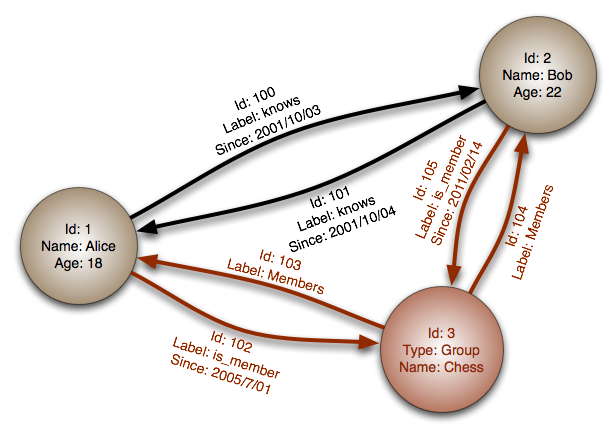
\includegraphics[width=.9\linewidth]{illustrations/GraphDatabase_PropertyGraph.png}		
	%   }
	\caption{Illustration d'une base de données NoSQL de type graphe. Source : \url{https://en.wikipedia.org/wiki/Graph_database}, consultée le $10/05/2019$}
	\label{fig:graphe-nosql}
\end{figure}
		\subparagraph{Document} Une base de données NoSQL de type document permet de stocker les données en reposant sur le paradigme clé-valeur. Toutefois, les valeur stockées sont complexes, il s'agit de documents de type JSON, XML, etc. L'accès aux données d'un enregistrement peut se faire de manière hiérarchique. La possibilité de stocker des objets complexes et hétérogènes  est un des points forts des bases de données NoSQL de type  document. Un exemple est fourni dans la Figure \ref{fig:document-nosql}. Une des différences majeures entre les bases de données clé-valeur et celles de type document c'est que pour les premières, l'indexation est au niveau  des clés seulement, tandis que pour les deuxièmes, l'indexation est au niveau clé et valeur. En pratique, pour les bases de données clé-valeur, les données sont récupérées en se basant sur la clé et pour les autres, la récupération d'un enregistrement peut être basée sur la clé et sur la valeur étant donné que la valeur est semi-structuré (valeur de type JSON, XML, etc.)
		\begin{figure}[h]
			\centering
				\resizebox{\textwidth}{!}{
			% Graphic for TeX using PGF
% Title: /home/hayat/RipeAtlasTraceroutesAnalysis/2019/Rapport_Mai/illustrations/document-nosql.dia
% Creator: Dia v0.97+git
% CreationDate: Tue May  7 11:56:16 2019
% For: hayat
% \usepackage{tikz}
% The following commands are not supported in PSTricks at present
% We define them conditionally, so when they are implemented,
% this pgf file will use them.
\ifx\du\undefined
  \newlength{\du}
\fi
\setlength{\du}{15\unitlength}
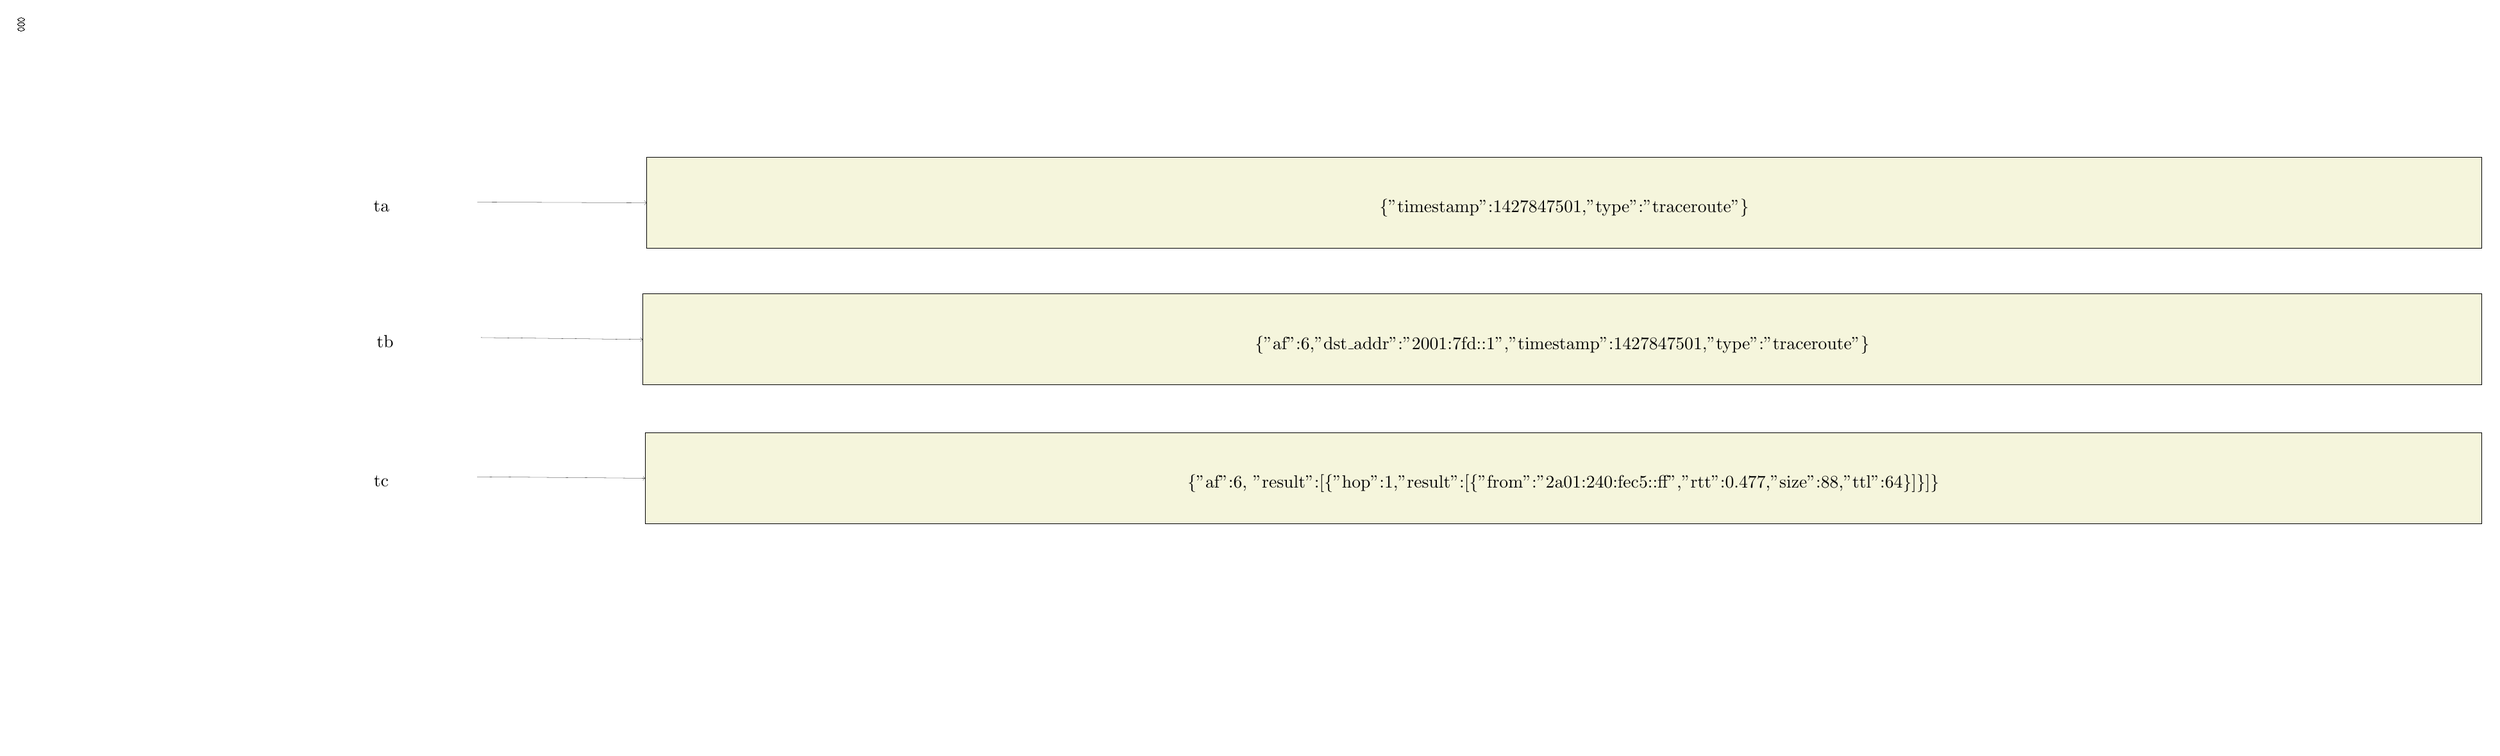
\begin{tikzpicture}[even odd rule]
\pgftransformxscale{1.000000}
\pgftransformyscale{-1.000000}
\definecolor{dialinecolor}{rgb}{0.000000, 0.000000, 0.000000}
\pgfsetstrokecolor{dialinecolor}
\pgfsetstrokeopacity{1.000000}
\definecolor{diafillcolor}{rgb}{1.000000, 1.000000, 1.000000}
\pgfsetfillcolor{diafillcolor}
\pgfsetfillopacity{1.000000}
\pgfsetlinewidth{0.000000\du}
\pgfsetdash{}{0pt}
\pgfsetmiterjoin
\definecolor{diafillcolor}{rgb}{0.960784, 0.960784, 0.960784}
\pgfsetfillcolor{diafillcolor}
\pgfsetfillopacity{1.000000}
\pgfpathellipse{\pgfpoint{7.395991\du}{3.752005\du}}{\pgfpoint{1.899011\du}{0\du}}{\pgfpoint{0\du}{1.012005\du}}
\pgfusepath{fill}
\definecolor{dialinecolor}{rgb}{0.000000, 0.000000, 0.000000}
\pgfsetstrokecolor{dialinecolor}
\pgfsetstrokeopacity{1.000000}
\pgfpathellipse{\pgfpoint{7.395991\du}{3.752005\du}}{\pgfpoint{1.899011\du}{0\du}}{\pgfpoint{0\du}{1.012005\du}}
\pgfusepath{stroke}
% setfont left to latex
\definecolor{dialinecolor}{rgb}{0.000000, 0.000000, 0.000000}
\pgfsetstrokecolor{dialinecolor}
\pgfsetstrokeopacity{1.000000}
\definecolor{diafillcolor}{rgb}{0.000000, 0.000000, 0.000000}
\pgfsetfillcolor{diafillcolor}
\pgfsetfillopacity{1.000000}
\node[anchor=base,inner sep=0pt, outer sep=0pt,color=dialinecolor] at (7.395991\du,3.947005\du){ta};
\pgfsetlinewidth{0.000000\du}
\pgfsetdash{}{0pt}
\pgfsetmiterjoin
\definecolor{diafillcolor}{rgb}{0.960784, 0.960784, 0.960784}
\pgfsetfillcolor{diafillcolor}
\pgfsetfillopacity{1.000000}
\pgfpathellipse{\pgfpoint{7.469011\du}{6.436015\du}}{\pgfpoint{1.899011\du}{0\du}}{\pgfpoint{0\du}{1.012005\du}}
\pgfusepath{fill}
\definecolor{dialinecolor}{rgb}{0.000000, 0.000000, 0.000000}
\pgfsetstrokecolor{dialinecolor}
\pgfsetstrokeopacity{1.000000}
\pgfpathellipse{\pgfpoint{7.469011\du}{6.436015\du}}{\pgfpoint{1.899011\du}{0\du}}{\pgfpoint{0\du}{1.012005\du}}
\pgfusepath{stroke}
% setfont left to latex
\definecolor{dialinecolor}{rgb}{0.000000, 0.000000, 0.000000}
\pgfsetstrokecolor{dialinecolor}
\pgfsetstrokeopacity{1.000000}
\definecolor{diafillcolor}{rgb}{0.000000, 0.000000, 0.000000}
\pgfsetfillcolor{diafillcolor}
\pgfsetfillopacity{1.000000}
\node[anchor=base,inner sep=0pt, outer sep=0pt,color=dialinecolor] at (7.469011\du,6.631015\du){tb};
\pgfsetlinewidth{0.000000\du}
\pgfsetdash{}{0pt}
\pgfsetmiterjoin
\definecolor{diafillcolor}{rgb}{0.960784, 0.960784, 0.960784}
\pgfsetfillcolor{diafillcolor}
\pgfsetfillopacity{1.000000}
\pgfpathellipse{\pgfpoint{7.394011\du}{9.196015\du}}{\pgfpoint{1.899011\du}{0\du}}{\pgfpoint{0\du}{1.012005\du}}
\pgfusepath{fill}
\definecolor{dialinecolor}{rgb}{0.000000, 0.000000, 0.000000}
\pgfsetstrokecolor{dialinecolor}
\pgfsetstrokeopacity{1.000000}
\pgfpathellipse{\pgfpoint{7.394011\du}{9.196015\du}}{\pgfpoint{1.899011\du}{0\du}}{\pgfpoint{0\du}{1.012005\du}}
\pgfusepath{stroke}
% setfont left to latex
\definecolor{dialinecolor}{rgb}{0.000000, 0.000000, 0.000000}
\pgfsetstrokecolor{dialinecolor}
\pgfsetstrokeopacity{1.000000}
\definecolor{diafillcolor}{rgb}{0.000000, 0.000000, 0.000000}
\pgfsetfillcolor{diafillcolor}
\pgfsetfillopacity{1.000000}
\node[anchor=base,inner sep=0pt, outer sep=0pt,color=dialinecolor] at (7.394011\du,9.391015\du){tc};
\pgfsetlinewidth{0.000000\du}
\pgfsetdash{}{0pt}
\pgfsetmiterjoin
{\pgfsetcornersarced{\pgfpoint{0.000000\du}{0.000000\du}}\definecolor{diafillcolor}{rgb}{0.960784, 0.960784, 0.862745}
\pgfsetfillcolor{diafillcolor}
\pgfsetfillopacity{1.000000}
\fill (12.651200\du,2.864010\du)--(12.651200\du,4.664010\du)--(49.000000\du,4.664010\du)--(49.000000\du,2.864010\du)--cycle;
}{\pgfsetcornersarced{\pgfpoint{0.000000\du}{0.000000\du}}\definecolor{dialinecolor}{rgb}{0.000000, 0.000000, 0.000000}
\pgfsetstrokecolor{dialinecolor}
\pgfsetstrokeopacity{1.000000}
\draw (12.651200\du,2.864010\du)--(12.651200\du,4.664010\du)--(49.000000\du,4.664010\du)--(49.000000\du,2.864010\du)--cycle;
}% setfont left to latex
\definecolor{dialinecolor}{rgb}{0.000000, 0.000000, 0.000000}
\pgfsetstrokecolor{dialinecolor}
\pgfsetstrokeopacity{1.000000}
\definecolor{diafillcolor}{rgb}{0.000000, 0.000000, 0.000000}
\pgfsetfillcolor{diafillcolor}
\pgfsetfillopacity{1.000000}
\node[anchor=base,inner sep=0pt, outer sep=0pt,color=dialinecolor] at (30.825600\du,3.959010\du){\{"timestamp":1427847501,"type":"traceroute"\}};
\pgfsetlinewidth{0.000000\du}
\pgfsetdash{}{0pt}
\pgfsetmiterjoin
{\pgfsetcornersarced{\pgfpoint{0.000000\du}{0.000000\du}}\definecolor{diafillcolor}{rgb}{0.960784, 0.960784, 0.862745}
\pgfsetfillcolor{diafillcolor}
\pgfsetfillopacity{1.000000}
\fill (12.570000\du,5.574010\du)--(12.570000\du,7.374010\du)--(49.000000\du,7.374010\du)--(49.000000\du,5.574010\du)--cycle;
}{\pgfsetcornersarced{\pgfpoint{0.000000\du}{0.000000\du}}\definecolor{dialinecolor}{rgb}{0.000000, 0.000000, 0.000000}
\pgfsetstrokecolor{dialinecolor}
\pgfsetstrokeopacity{1.000000}
\draw (12.570000\du,5.574010\du)--(12.570000\du,7.374010\du)--(49.000000\du,7.374010\du)--(49.000000\du,5.574010\du)--cycle;
}% setfont left to latex
\definecolor{dialinecolor}{rgb}{0.000000, 0.000000, 0.000000}
\pgfsetstrokecolor{dialinecolor}
\pgfsetstrokeopacity{1.000000}
\definecolor{diafillcolor}{rgb}{0.000000, 0.000000, 0.000000}
\pgfsetfillcolor{diafillcolor}
\pgfsetfillopacity{1.000000}
\node[anchor=base,inner sep=0pt, outer sep=0pt,color=dialinecolor] at (30.785000\du,6.669010\du){\{"af":6,"dst\_addr":"2001:7fd::1","timestamp":1427847501,"type":"traceroute"\}};
\pgfsetlinewidth{0.000000\du}
\pgfsetdash{}{0pt}
\pgfsetmiterjoin
{\pgfsetcornersarced{\pgfpoint{0.000000\du}{0.000000\du}}\definecolor{diafillcolor}{rgb}{0.960784, 0.960784, 0.862745}
\pgfsetfillcolor{diafillcolor}
\pgfsetfillopacity{1.000000}
\fill (12.620000\du,8.324010\du)--(12.620000\du,10.124010\du)--(48.995000\du,10.124010\du)--(48.995000\du,8.324010\du)--cycle;
}{\pgfsetcornersarced{\pgfpoint{0.000000\du}{0.000000\du}}\definecolor{dialinecolor}{rgb}{0.000000, 0.000000, 0.000000}
\pgfsetstrokecolor{dialinecolor}
\pgfsetstrokeopacity{1.000000}
\draw (12.620000\du,8.324010\du)--(12.620000\du,10.124010\du)--(48.995000\du,10.124010\du)--(48.995000\du,8.324010\du)--cycle;
}% setfont left to latex
\definecolor{dialinecolor}{rgb}{0.000000, 0.000000, 0.000000}
\pgfsetstrokecolor{dialinecolor}
\pgfsetstrokeopacity{1.000000}
\definecolor{diafillcolor}{rgb}{0.000000, 0.000000, 0.000000}
\pgfsetfillcolor{diafillcolor}
\pgfsetfillopacity{1.000000}
\node[anchor=base,inner sep=0pt, outer sep=0pt,color=dialinecolor] at (30.807500\du,9.419010\du){\{"af":6, "result":\ensuremath{[}\{"hop":1,"result":\ensuremath{[}\{"from":"2a01:240:fec5::ff","rtt":0.477,"size":88,"ttl":64\}\ensuremath{]}\}\ensuremath{]}\}};
\pgfsetlinewidth{0.100000\du}
\pgfsetdash{}{0pt}
\pgfsetbuttcap
{
\definecolor{diafillcolor}{rgb}{0.000000, 0.000000, 0.000000}
\pgfsetfillcolor{diafillcolor}
\pgfsetfillopacity{1.000000}
% was here!!!
\pgfsetarrowsend{to}
\definecolor{dialinecolor}{rgb}{0.000000, 0.000000, 0.000000}
\pgfsetstrokecolor{dialinecolor}
\pgfsetstrokeopacity{1.000000}
\draw (9.295000\du,3.752010\du)--(12.651200\du,3.764010\du);
}
\pgfsetlinewidth{0.100000\du}
\pgfsetdash{}{0pt}
\pgfsetbuttcap
{
\definecolor{diafillcolor}{rgb}{0.000000, 0.000000, 0.000000}
\pgfsetfillcolor{diafillcolor}
\pgfsetfillopacity{1.000000}
% was here!!!
\pgfsetarrowsend{to}
\definecolor{dialinecolor}{rgb}{0.000000, 0.000000, 0.000000}
\pgfsetstrokecolor{dialinecolor}
\pgfsetstrokeopacity{1.000000}
\draw (9.368020\du,6.436010\du)--(12.570000\du,6.474010\du);
}
\pgfsetlinewidth{0.100000\du}
\pgfsetdash{}{0pt}
\pgfsetbuttcap
{
\definecolor{diafillcolor}{rgb}{0.000000, 0.000000, 0.000000}
\pgfsetfillcolor{diafillcolor}
\pgfsetfillopacity{1.000000}
% was here!!!
\pgfsetarrowsend{to}
\definecolor{dialinecolor}{rgb}{0.000000, 0.000000, 0.000000}
\pgfsetstrokecolor{dialinecolor}
\pgfsetstrokeopacity{1.000000}
\draw (9.293020\du,9.196010\du)--(12.620000\du,9.224010\du);
}
% setfont left to latex
\definecolor{dialinecolor}{rgb}{0.000000, 0.000000, 0.000000}
\pgfsetstrokecolor{dialinecolor}
\pgfsetstrokeopacity{1.000000}
\definecolor{diafillcolor}{rgb}{0.000000, 0.000000, 0.000000}
\pgfsetfillcolor{diafillcolor}
\pgfsetfillopacity{1.000000}
\node[anchor=base west,inner sep=0pt,outer sep=0pt,color=dialinecolor] at (9.850000\du,14.350000\du){};
\end{tikzpicture}

		}
			\caption{Illustration d'une base de données NoSQL de type document}
			\label{fig:document-nosql}
		\end{figure}
		\subparagraph{Colonnes} Dans les bases de données traditionnelles, les données sont stockées sur des lignes. Dans le cas d'une base NoSQL orientée colonne, les données sont stockées par colonne. L'interrogation de ce type de bases travaille sur une colonne particulière sans devoir passer par les autres colonnes comme dans les bases de données relationnelles classiques. Une base de données de type colonne est adaptée pour les requêtes analytiques comme les requêtes d'agrégation (moyennes, maximum, etc). La Figure \ref{fig:comomn-nosql} illustre la différence entre le stockage dans une base de données relationnelle et une base de données orientée colonnes\footnote{Cette illustration  est basée sur une figure disponible sur \url{https://www.illustradata.com/bases-nosql-orientees-colonnes-quest-cest}, consulté le $02/05/2019$.}. 
		Les bases de données NoSQL orientées colonnes sont conçues pour pouvoir ajouter facilement de nouveaux colonnes, jusqu'à des millions de colonnes. De plus, le coût du stockage de \textit{null} vaut $ 0 $.
		
	\begin{figure}[h]
		\centering
		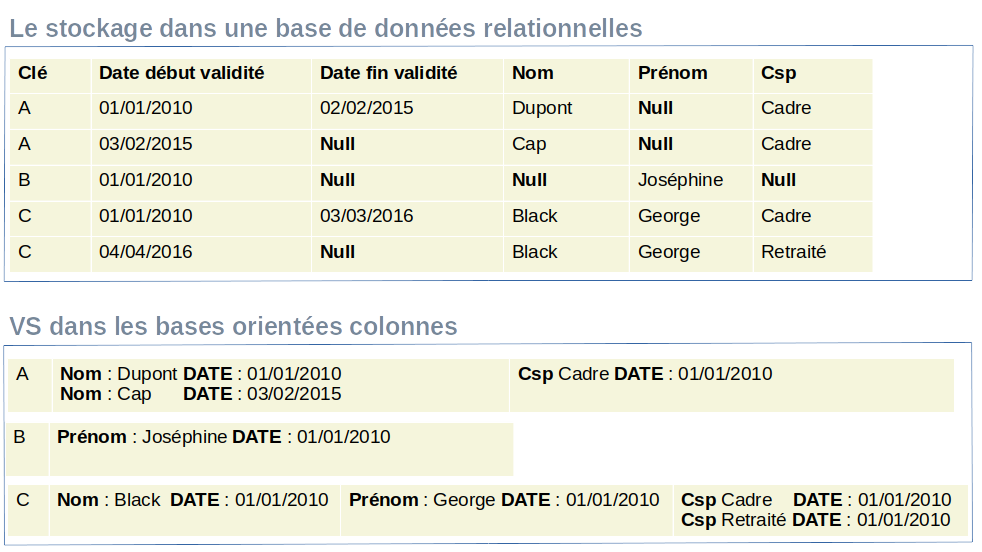
\includegraphics[width=\linewidth]{illustrations/colomn-db-2.png}
		\caption{Illustration d'une base de données NoSQL de type colonne}
		\label{fig:comomn-nosql}
	\end{figure}


Les bases de données NoSQL sont conçues pour répondre à des besoins spécifiques. Elles n'ont pas été créées pour remplacer les bases de données relationnelles. Il existe plusieurs implémentations des quatre types des bases de données NoSQL. Chaque implémentation favorise un ou plusieurs  éléments suivants : la disponibilité des données, la cohérence des données et la tolérance au partitionnement.  C'est ce qu'explique le théorème CAP.	
		\paragraph{Big Data et le théorème  CAP} \label{par:cap-theorem}:
		
		Dans le but d'assurer un traitement rapide de données à grande échelle, ces dernières sont réparties sur un cluster de machines  (appelées aussi  n\oe{}uds). Le théorème CAP annonce que dans le cadre d'un système distribué où le stockage de données est  réparti sur plusieurs machines,
		%(ou n\oe{}uds) (voir \ref{sec:distruted-camput}),  
		une base de données ne peut pas garantir les trois attributs suivants : \textit{Consistency}, \textit{Availability} et \textit{Partition Tolerence}  en même temps. \par
			\textbf{Consistency (ou intégrité)} Chaque donnée a un seul état visible depuis l'extérieur. Par exemple, les différents serveurs hébergeant la base de données voient tous les mêmes données. C'est pourquoi une lecture faite après une écriture doit renvoyer la donnée précédemment écrite. \par
			\textbf{Availability (ou disponibilité)} Une base de données doit toujours fournir une réponse à une requête d'un client.\par
			%En cas d'une panne technique sur un des serveurs qui hébergent  la base de données, il faut s'assurer de desservir  des clients.  Généralement, cela est assuré à travers la réplication des données
			 \textbf{Partition tolerance (ou  tolérance au partitionnement) } Une coupure du réseau entre deux n\oe{}uds ou l'indisponibilité d'un de ces n\oe{}uds ne devrait pas affecter le bon fonctionnement du système. Tout de même,  ce dernier doit répondre à la demande d'un client. 

		
		%conclusion
		Les trois attributs du théorème CAP s'opposent entre eux. On distingue les trois scénarios possibles:
		
		\begin{itemize}
			\item [--] Le couple \textbf{CA} : les SGBDR adoptent les deux attributs C et A, qui sont une forte cohérence et disponibilité. Cependant, l'attribut partitionnement réseau n'est pas toujours pris en compte.
			\item [--] Le couple \textbf{CP} : les implémentations du C et du P assurent la tolérance aux pannes en distribuant les données sur plusieurs serveurs. Malgré cette réplication, ces implémentations assurent la cohérence des données même en présence de mises à jour concurrentielles.
			\item [--] Le couple \textbf{AP} : les implémentations du A et du  P assurent un temps de réponse rapide et une réplication de données. Cependant, les mises à jour étant asynchrones, la garantie que la version d'une donnée soit bonne, ne peut pas être assurée.
			
		\end{itemize}
		
		La Figure \ref{fig:cap} présente des implémentations des différents types de bases de données NoSQL pour chaque couple CA, CP et AP.
		
		\begin{figure}[h]
			\centering
			\captionsetup{justification=centering}
			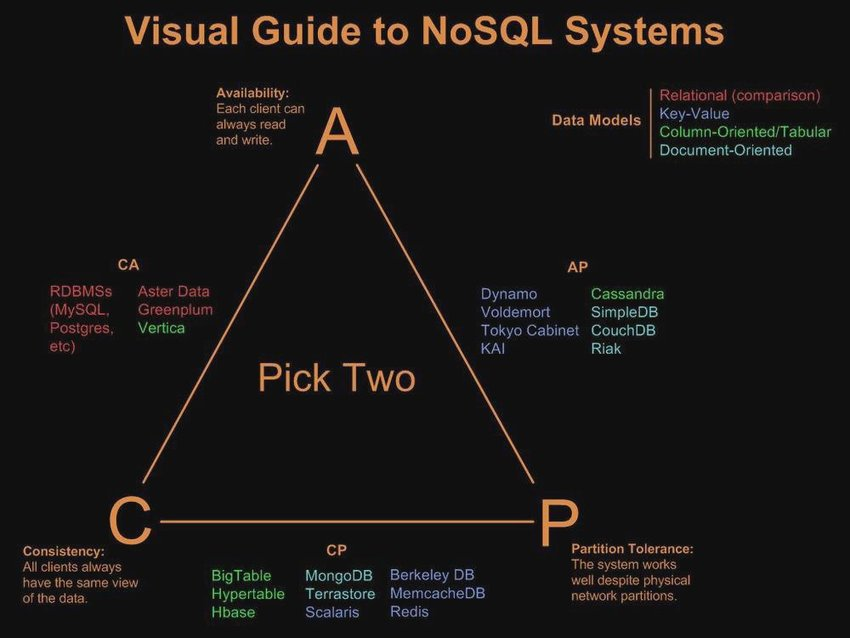
\includegraphics[width=1\linewidth]{illustrations/cap}
			\caption{Bases de données NoSQL suivant le théorème de CAP }
			\label{fig:cap}
			\source{\url{https://www.researchgate.net/figure/CAP-theorem-concept-5-II-WHY-YOU-NEED-NOSQL-The-first-reason-to-use-NoSQL-is-because_fig2_323309389}, consultée le $05/08/2018$.}
		\end{figure}
		
		
		
		Le choix d'une base de données relationnelle ou NoSQL dépend des besoins des entreprises. En terme de tendances, la Figure \ref{fig:ranking-db} reprend un classement des SGBDs au $1$ août $ 2018 $. La suite de la liste ainsi que  la méthode qui dirige ce classement sont    disponibles sur le site  Web \textit{DB-Engines Ranking}\footnote{URL : \url{https://db-engines.com/},  consulté le $01/08/2018$.}. Parmi les critères du classement, on trouve le nombre de références du SGBD sur les sites Internet. 
		
		%Ce nombre de référence est quantifiable à partir du  nombre lui-même de résultats obtenus des différents moteurs de recherche comme Google, Bing, etc. 
		
		\begin{figure}[h]
			\centering
			\captionsetup{justification=centering}
			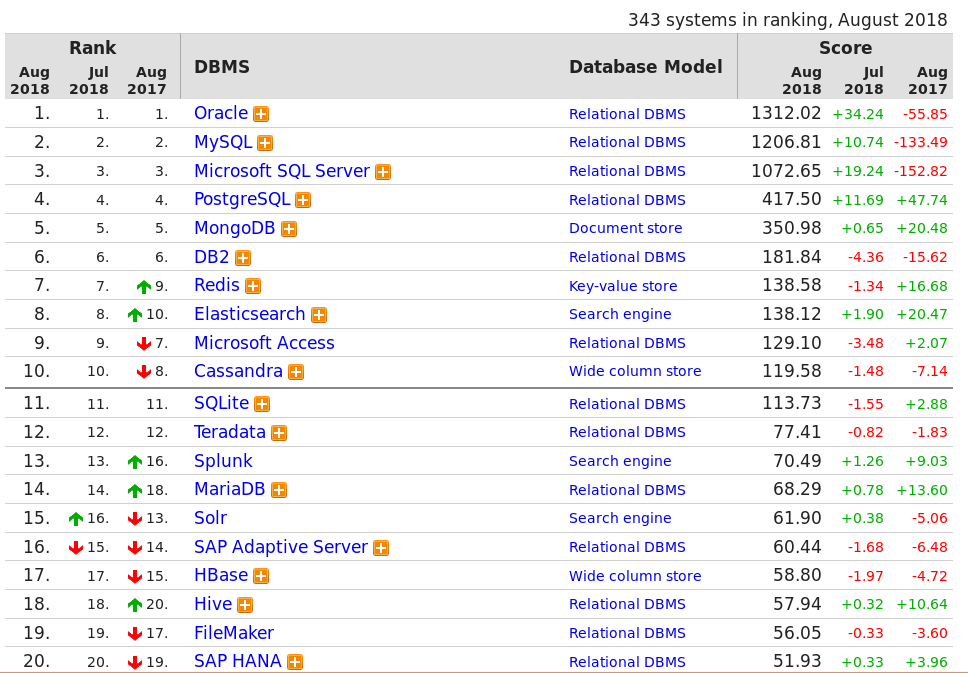
\includegraphics[width=1\linewidth]{illustrations/ranking-db}
			\caption{Un classement des SGBDs sur \textit{DB-Engines Ranking} du $1$ août $2018$ }
			\label{fig:ranking-db}
			\source{\url{https://db-engines.com/en/ranking}, consultée le $01/08/2018$.}
		\end{figure}
		
		\subsection{Extraction, Transformation, Loading (ETL)} \label{sec:etl}
		Dans une même organisation, il est possible d'avoir plusieurs sources de données~: des bases de données relationnelles, des bases de données NoSQL, des fichiers de données de type Excel, etc. 
		Dans le cas où une analyse de données devrait impliquer des données en provenance de  sources  de données hétérogènes, il est nécessaire de faire appel aux opérations ETL :
		
		\textbf{Extraction} :  la diversité des sources de données implique des formats de données différents. Généralement, ce sont des données en provenance des bases de données relationnelles, des fichiers plats, des bases de données non relationnelles,  etc. Le but de la phase d'extraction est de convertir les données en un seul format approprié à l'étape de la transformation. Cette phase  vérifie si les données respectent  une structure attendue. Si ce n'est pas le cas, les données peuvent être totalement ou partiellement rejetées.
		
		\textbf{Transformation} : cette étape  s'applique  sur les données extraites. Elle comprend  une série de règles ou de fonctions. Ces derniers sont appliqués sur les données avant de les envoyer vers la cible. Certaines sources de données nécessitent  peu de transformations, voire aucune. Dans d'autres cas, un ou plusieurs  types de transformation sont  nécessaires. Quelques exemples de transformations  sont    listées ci-dessous :
		\begin{itemize}
			\item sélection d'un nombre  de colonnes à charger parmi plusieurs colonnes;
			\item adaptation des codes. Par exemple,  quand le système de stockage source utilise 1 pour dénoter un homme et l'entrepôt de données cible  utilise "H"; 
			\item conversion des devises, c'est le cas par exemple où les salaires sont exprimés en une devise différente de l'euro;
			\item élimination des doublons.
		\end{itemize}
		
		\textbf{Loading} : l'objectif de cette étape est de charger les données transformées vers l'entrepôt de données. Le chargement des données dépend des besoins de l'organisation. Dans certains cas, on prévoit le remplacement des informations existantes par des informations cumulatives plus récentes. Dans d'autres cas, les nouvelles informations sont ajoutées dans la suite de celles existantes. 
		
		En ce qui concerne la fréquence  des opérations ETL, elles peuvent être planifiées de manière horaire, quotidienne, hebdomadaire, mensuelle ou autre.
		
		 %ETL est un système de chargement de données depuis les différentes sources de données jusqu'à l'entrepôt de données. Ce système  s'occupe de faire passer les données par un ensemble de traitements pour les nettoyer,  les contextualiser et enfin les charger. Les tâches ETL prennent énormément du temps dans un projet d'analyse de données. Il est important d'assurer  la qualité de données et d'éviter les fausses données ou les données inutiles. 
		 
		
		
		
		\subsection{Schema on Write VS Schema on Read} \label{sec:schema-read-write}
		
		Lors du chargement des données depuis leurs sources de stockage, on distingue deux approches : \textit{ Schema on Write} et \textit{Schema on Read}.
		% L'approche \textit{Schema on Read } est celle utilisée par l'outil Amazon Athena présenté dans la section \ref{par:allservices}.
		
		Dans la première, il faut définir les colonnes, le format de données, les types, etc. La lecture des données est rapide et moins coûteuse étant donné l'effort entrepris pour définir la structure. C'est le cas des bases de données relationnelles.
		
		Dans la deuxième, les données sont chargées telles qu'elles sont, sans transformations ou changements. L'interprétation de ces données se fait lors de la lecture, et cela dépend des besoins pour lesquels les données sont analysées. Ainsi, les mêmes données peuvent être lues de différentes manières. Par exemple, l'action  de lire les données  d'une colonne, qu'elles soient de type entier ou bien chaîne de caractère d'un fichier CSV est la même, c'est le type de la donnée qui diffère. C'est l'approche utilisée par Amazon Athena (voir la section \ref{aws:athena}). 
		
\paragraph{Exemple illustratif}~

 Afin de montrer la différence entre les deux approches, nous comparons Apache Spark (présenté en détail dans la section \ref{apache-spark}) avec une base de données relationnelle (SQL Server).   Les étapes suivantes concernent  SQL Server:
%\begin{tcolorbox}{SQL RDBMS : exemple de SQL Server}
\begin{enumerate}
	\item Créer la table Traceroutes :
\begin{lstlisting}[language = sql, basicstyle=\small]
CREATE TABLE Traceroutes(
	id INT,
	dst_name VARCHAR(30),
	...
)
\end{lstlisting}
		
	\item  Charger les données depuis le fichier \textit{traceroute-2019-04-08T0000.json} vers la table Traceroutes, chaque ligne du fichier doit correspondre à la  structure  créée à l'étape $ 1 $:
\begin{lstlisting}[language = sql, basicstyle=\small]
BULK INSERT  Traceroutes
FROM 'c:\traceroutes\traceroute-2019-04-08T0000.csv'
WITH ROWTERMINATOR = '\n'
\end{lstlisting}
	
	\item Interroger les données : à l'issue de l'étape $2$,  les données sont chargées et prêtes à l'interrogation: 
\begin{lstlisting}[language = sql, basicstyle=\small]
SELECT dst_name FROM  Traceroutes
\end{lstlisting}
	\end{enumerate}

Pour les bases de données relationnelles, qui adoptent l'approche \textit{Schema on Write}, on ne peut pas ajouter des données avant de créer le schéma dirigeant ces dernières. De plus, la création du schéma nécessite la compréhension  exhaustive des données. 
Car en cas d'un changement du contenu du fichier de données, en terme de structure, la table créée doit être supprimée, mise à jour, ensuite il faut recharger à nouveau les données. L'implication de la mise à jour du schéma peut être coûteuse en terme de temps  dans le cas  d'un  volume de donnée  important, de l'ordre de plusieurs centaines de téraoctets. Dans certains cas, une mise à jour des relations avec d'autres tables est requise.

En ce qui concerne l'approche \textit{Schema on Read}, nous prenons l'exemple d'Apache Spark présenté en détail dans la section \ref{apache-spark}. En utilisant cette technologie, on crée un schéma selon les besoins de l'analyse de ces données.
% et non pas pour que la structure des données soit exactement celle à créer, sauf si cela fait partie des besoins. 
%Par exemple, on peut créer une table dont les colonnes correspondent  seulement à la moitié des colonnes possibles. Un autre exemple concerne l'utilisation  des conditions; on crée une table et durant le chargement des données, on ne charge que celles vérifiant une condition donnée. Pour AWS Athena et les autres technologies qui se basent sur  cette approche, les données sont chargées au moment de l'utilisation et avec plus de flexibilité.
Pour illustrer cette approche, l'annexe \ref{exemple-traceroute} présente une réponse d'une requête traceroute. Pour les besoins de l'outil de détection (voir le chapitre \ref{chap:algorith-detection}), plusieurs attributs ne sont pas pertinents. Ainsi, il est inutile de les charger lors de l'analyse.   En Spark, les données sont lues en associant les attributs d'une classe aux attributs de la réponse traceroute; c'est la classe Traceroute décrite dans le Listing \ref{lst:case-class-Traceroute}. En résultat, seules les données utiles qui sont chargées en mémoire pour qu'elles soient traitées.

La meilleure approche dépend des besoins de l'analyse. La première approche est meilleure en performances, en revanche, la deuxième est tolérante aux erreurs  humaines.

		\subsection{L'informatique distribuée et l'analyse de données massives} \label{sec:distruted-camput}
		Il existe deux stratégies pour appliquer des traitements sur un grand ensemble de données: 
		
		
		\begin{itemize}
			\item[--] Par distribution des traitements (\textit{scaling} des traitements)~: les traitements sont distribués sur un nombre de n\oe{}uds important. De ce fait, les données sont amenées jusqu'à ces n\oe{}uds.
			
			\item[--] Par distribution des données (\textit{scaling} des données)~: les données sont distribuées sur un nombre important de n\oe{}uds. Par ailleurs cela permet  de stocker un maximum de données. Il s'agit d'amener les traitements aux machines sur lesquelles les données sont stockées. Du fait que le stockage de données est réparti sur plusieurs machines, il est possible de traiter des données très volumineuses en un temps optimal. La première mise en \oe{}uvre de cette approche est le schéma MapReduce (voir la section  \ref{mapreducesection}). 
		\end{itemize}
\subsection{MapReduce} \label{mapreducesection}
%https://softwareengineering.stackexchange.com/questions/220605/why-big-data-needs-to-be-functional

MapReduce est un modèle de programmation proposé par Google. Il est conçu pour   le traitement distribué de grands ensembles de données   sur un cluster de machines. Un programme MapReduce est composé de deux phases principales   \textit{Map} et  \textit{Reduce}.

MapReduce divise le travail en petites parties, chacune pouvant être effectuée en parallèle sur le cluster de machines. Autrement dit, le  problème est divisé en un grand nombre de problèmes plus petits, chaque petit problème est traité pour donner des résultats individuelles. Ces résultats sont ensuite traités pour donner un résultat final. 
%Hadoop MapReduce est évolutif et peut également être utilisé sur de nombreux ordinateurs. 
%\begin{tcolorbox}
%	\textit{ MapReduce est un patron d'architecture de développement informatique, inventé par Google, dans lequel sont effectués des %calculs parallèles, et souvent distribués, de données potentiellement très volumineuses, typiquement supérieures en taille à 1 %téraoctet} \footnote{Source : \url{https://fr.wikipedia.org/wiki/MapReduce}, consultée le $20/12/2018$.}. 
%\end{tcolorbox}
La Figure 	\ref{fig:2-figure1-1-map-reduce-workflow} représente une vue d'ensemble du modèle de programmation MapReduce. 

\begin{figure}[h]
	\centering
	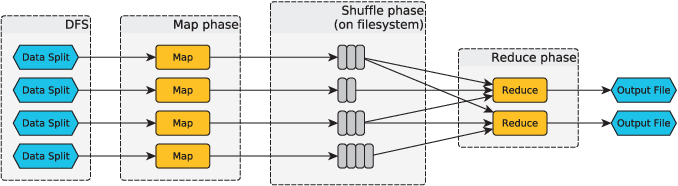
\includegraphics[width=\linewidth]{illustrations/2-Figure1-1-map-reduce-workflow}
	\caption{Vue d'ensemble du modèle MapReduce. Source : \cite{6427487}}
	\label{fig:2-figure1-1-map-reduce-workflow}
\end{figure}


Le modèle de données de base dans MapReduce  est la paire clé/valeur. Pendant la phase de \textit{Map}, la fonction  associée  au Map est exécutée sur chaque paire clé/valeur (K1,V1) des données d'entrée (\textit{Data Split}), ce que produit   une liste des paires clé/valeur (List(K2,V2)) intermédiaires pour chaque clé/valeur (K1,V1). Il existe une autre phase entre  \textit{Map} et de \textit{Reduce}, c'est la phase de \textit{Shffling}. Durant cette dernière,  les paires clé/valeur (List(K2,V2))  intermédiaire sont triées et regroupées par la clé. Il en résulte un ensemble de paires clé/valeur (K2, List(V2)) où chaque paire contient toutes les valeurs associées à une clé particulière (K2). Ces paires clé/valeur sont ensuite partitionnées et regroupées sur la clé, puis passée à la phase Reduce au cours de laquelle la fonction de réduction est appliquée individuellement à chaque clé et aux valeurs associées pour cette clé (K2,List(V2)). La phase \textit{Reduce} peut produire une valeur nulle ou une sortie (List(K3,V3)).

\section{Parcours de quelques technologies du Big Data}
La liste des technologies  du Big Data est en expansion continue pour répondre au mieux aux besoins de l'analyse de données massives. C'est pourquoi nous allons parcourir une liste non exhaustive des technologies liées au Big Data. En particulier, ce sont les technologies expérimentées pour analyser les traceroutes en provenance du projet Atlas.

MongoDB est la base de données NoSQL utilisée dans l'implémentation du travail de référence \cite{InternetHealthReport}. Amazon DynamoDB est la première technologie Big Data que nous avons utilisé pour réécrire l'outil de détection, ensuite, nous avons évalué la combinaison de trois services Web d'Amazon S3, Glue et Athena. Enfin, nous avons reproduit l'outil de détection en Spark/Scala. Pour Amazon Elastic MapReduce, nous l'avons utilisé pour exécuter l'application Spark/Scala dans un cluster de machines. Nous présentons aussi l'écosystème Hadoop, étant donné qu'il fait partie des principales plateformes du Big Data.
	
\subsection{MongoDB} \label{subsubsection:mongodb}
%	\paragraph{Introduction à la base de données MongoDB} \label{subsubsection:mongodb}~
MongoDB\footnote{URL : \url{https://www.mongodb.com/}, consulté le $02/08/2018$.} est une base de données  NoSQL de type Document\footnote{Une base de données NoSQL de type document est décrite dans la section \ref{sec:nosql-database}.}.  MongoDB est classé parmi les  SGBDs adoptant le couple CP (Consistency et Partition Tolerance) dans le théorème  CAP\footnote{Le théorème  CAP est décrit dans la section \ref{par:cap-theorem}}. Une base de données créées dans MongoDB est un ensemble de collections. Une collection dans MongoDB est équivalente à une table dans un SGBDR.
	
En $ 2016 $, MongoDB devient disponible en mode cloud sous le nom  MongoDB Atlas \footnote{URL : \url{https://www.mongodb.com/cloud/atlas}, consulté le $ 02/08/2018 $.}.  Il est distribué à travers les trois fournisseurs du cloud: Amazon Web Services (AWS), Google Cloud Platform et Microsoft Azure.  En terme de tarifs, plusieurs formules sont proposées \footnote{Source : \url{https://www.mongodb.com/cloud/atlas/pricing}, consultée le $ 02/08/2018 $.}, y inclut l'offre gratuite pour expérimenter MongoDB Atlas.  Les frais d'utilisation du service MongoDB Atlas dépendent du stockage, de la  RAM allouée et des options choisies. Les documents sont stockés dans MongoDB sous format BSON.
	
\begin{tcolorbox}
	BSON (ou Binary JSON) est un format utilisé pour stocker et transférer les données dans la base de données MongoDB. BSON facilite la représentation des structures de données simples et des tableaux associatifs\footnote{Source : \url{https://fr.wikipedia.org/wiki/BSON}, consultée le $ 02/08/2018 $.}.
\end{tcolorbox}
	
	\subsection{Amazon DynamoDB}\label{aws:dynmo}~
	
	% \paragraph{Amazon DynamoDB :}\label{aws:dynmo}~
	
	Amazon DynamoDB\footnote{URL : \url{https://aws.amazon.com/fr/dynamodb/}, consulté le $02/05/2018$.} est une base de données NoSQL de type clé-valeur distribuée, gérée par les services d'Amazon. Elle est capable de stocker un volume important de données limité par la capacité de l'infrastructure d'AWS. Amazon DynamoDB   est un service  simple et facile à utiliser,  il ne nécessite aucune configuration préalable. 
	
	Amazon DynamoDB  est une base de données évolutive permettant à l'utilisateur final de passer à l'échelle facilement et rapidement. Cette technologie offre des performances constantes à une échelle essentiellement infinie, limitée uniquement par la taille physique du cloud AWS. Amazon DynamoDB est flexible. Aucun schéma n'est requis pour stocker les données. Les frais d'utilisation de ce service dépendent de trois éléments\footnote{Source : \url{https://aws.amazon.com/fr/dynamodb/pricing/}, consultée $02/05/2018$.}:
	\begin{itemize}
		\item[--] la quantité de données stockées : DynamoDB est facturé par Go d'espace disque utilisé ($ 0,250 $ USD par Go par mois);
		\item[--] la capacité en lecture par seconde ($ 0,470 $ USD par unité de capacité d'écriture par mois);
		\item[--]  la capacité en écriture par seconde ($ 0,090 $ USD par unité de capacité de lecture par mois);
	\end{itemize}

\subsection{Amazon S3, Amazon Glue et Amazon Athena }

La combinaison d'Amazon S3, Amazon Glue et Amazon Athena permet de créer un environnement Big Data capable d'assurer respectivement le stockage de données, le chargement de données  et l'interrogation de données. 

%\paragraph{Introduction aux services Amazon S3, Amazon Athena et Amazon Glue }

\paragraph{Amazon S3}
\footnote{URL : \url{https://aws.amazon.com/fr/s3/}, consulté le $06/07/2018$.} est un service de stockage d'objets dans le cloud. Il est conçu pour stocker et  récupérer toute quantité de données. Il peut assurer $ 99,999999999 $ \% de durabilité. La sécurité  et l'accès aux données sont assurés. Il existe plusieurs classes de stockage qui répondent aux différents besoins. 

Dans Amazon S3, le fichier à stocker et considéré comme objet. Un objet est référencé par une clé qui reprend d'abord le chemin vers un pseudo répertoire suivi par  le nom de l'objet.  Le terme pseudo répertoire est utilisé car, en réalité, Amazon S3 ne stocke pas les objets dans des dossiers comme le cas d'un système d'exploitation. Chaque objet appartient à un compartiment, un compartiment appartient aussi à une des régions d'Amazon et le nom d'un compartiment est unique. Prenons l'exemple d'un  compartiment \textit{foo}, contenant deux objets ayant respectivement les clés \textit{A/b/c/i.txt} et \textit{A/b/d/k.txt}, dans ce cas, ces deux objets ne partagent que le même compartiment.
%Les fichiers des données sont organisés dans ce qu'on appelle un compartiment, c'est une simulation de dossier dans un système d'exploitation. A l'intérieur d'un compartiment, il est possible de créer des compartiments imbriqués. C'est une simulation d'arborescence de dossiers car physiquement cet arborescence n'existe pas. En ce qui concerne les frais du service AWS S3, . 
Le Tableau   	\ref{tab:pricing-s3-standard} décrit les tarifs de la formule standard relative à un mois.
\begin{table}[H]
	\centering
	\captionsetup{justification=centering}
	\begin{tabular}{l c }
		\textbf{Région} & UE (Irlande) \\ \hline
		\textbf{Première tranche de $ 50 $ To} &	$ 0,023 $ USD par Go\\ \hline
		\textbf{$ 450 $ To suivants} &	$ 0,022 $ USD par Go \\ \hline
		\textbf{Plus de $ 500 $ To} &	$ 0,021 $ USD par Go\\ \hline
	\end{tabular}
	\caption{Les tarifs du AWS S3 (formule Stockage standard S3)}
	\label{tab:pricing-s3-standard}
	\source{\url{https://aws.amazon.com/fr/s3/pricing/}, consultée le $05/08/2018$.}
\end{table}


\paragraph{Amazon  Glue} \label{aws:glue}
\footnote{URL : \url{https://aws.amazon.com/fr/glue/}, consulté le $06/07/2018$.} est un service d'extraction, de transformation et de chargement. L'objectif de ce service est de découvrir les données, les transformer et les rendre accessibles à la recherche et à l'interrogation.  Amazon Glue  est utile pour la construction des entrepôts de données; il découvre les métadonnées relatives aux magasins de données et les rend accessibles dans un catalogue central. En prenant en entrée les données  présentes dans un compartiment dans Amazon S3, Amazon Glue découvre le schéma de ces données. Il dispose de plusieurs classificateurs intégrés pour la découverte des données. Par exemple un classificateur pour trouver le schéma  de données en format JSON, XML, etc. Si les classificateurs intégrés ne répondent pas aux besoins particuliers, il est possible de créer des classificateurs personnalisés. 

Les frais de ce service dépendent du temps écoulé lors de l'analyse des données par les robots d'analyse durant la découverte du schéma. A ces frais s'ajoutent les frais du catalogue de données qui va être peuplé par les résultats fournis par les robots de l'analyse. Par exemple, on paye $ 0,44 $ USD par heure par DPU\footnote{DPU : unité de traitement des données.}, il est facturé à la seconde avec un minimum de $ 10 $ minutes par robot d'analyse exécuté. Plus de détails sont disponibles sur le site Web d'Amazon Glue\footnote{Source : \url{https://aws.amazon.com/fr/glue/pricing/}, consultée le $05/08/2018$.}.

\paragraph{Amazon Athena}\label{aws:athena}\footnote{URL : \url{https://aws.amazon.com/fr/athena/}, consulté le $06/07/2018$.} est un service de requêtes  interactif. Il permet d'interroger les données présentes dans Amazon S3 avec des requêtes SQL plus avancées. Le service Amazon Athena est considéré comme \textit{serverless}. Amazon Athena utilise l'approche \textbf{\textit{schema-on-read}} (voir la section \ref{sec:schema-read-write}) afin de projeter le schéma donné en entrée sur les données au moment de l'exécution de la requête SQL demandée. Le schéma sur lequel les données peuvent être projetées peut être créé manuellement ou bien utiliser le catalogue créé dans Amazon Glue.
Le service Amazon Athena est facturé suivant la quantité de données analysée. Précisément, $ 5 $ USD par To de données analysées.


\begin{tcolorbox}
	Une \textbf{\textit{requête est	interactive}} si on peut  obtenir immédiatement une réponse à la requête.  Dans le cas échéant, les résultats sont obtenus  dans le cadre d'un code source pour un des langages de programmation, typiquement à travers une API.
\end{tcolorbox}

\begin{tcolorbox}
	\textbf{\textit{Serverless}} peut être décomposé en \textit{server} et \textit{less}. Un outil est \textit{serverless} quand l'utilisateur final de cet outil peut l'utiliser sans se soucier de toute configuration ou gestion des serveurs derrière ce service. D'après Amazon\footnote{URL : \url{https://aws.amazon.com/serverless/}, consultée le  $05/08/2018$.},  \textit{Serverless} est l'architecture native du cloud.
\end{tcolorbox}

L'exécution des requêtes SQL est effectuée par le moteur de requêtes SQL Presto. Pour les instruction DDL (Data Definition Language), elles sont effectuées par  \textit{Hive Data Definition Language} \footnote{URL : \url{https://cwiki.apache.org/confluence/display/Hive/LanguageManual+DDL}, consulté le $05/08/2018$.}. Les requêtes DDL incluent la création, la suppression et la mise à jour de la structure de la table dans le cas d'une base de données relationnelles, d'une collection, d'une vue, etc. 

\begin{tcolorbox}
	\textbf{Hive Data definition language} (DLL) est un sous-ensemble de déclarations qui décrivent la structure de données dans Apache Hive.  Principalement, ce sont les instruction de création, suppression et de mise à jour de la structure des objets comme les bases de données, les tables, les vues et autres.
\end{tcolorbox}

\begin{tcolorbox}
	\textbf{\textit{Presto\footnote{URL : \url{http://prestodb.io/}, consulté le $01/08/2018$.} }} est un moteur de requêtes SQL open source destiné au Big Data. Il permet d'exécuter des requêtes analytiques interactives sur des données de taille importante; jusqu'à des pétaoctets de données.
	Presto interroge les données où elles sont hébergées. Ceci inclut les bases de données relationnelles, Amazon S3 et autres dépôts propriétaires. De plus, une même requête SQL peut combiner plusieurs sources de données. C'est intéressant pour les organisations ayant plusieurs sources de données.% Il fournit les résultats en quelques secondes, voire quelques minutes.  Il supporte les types de données complexes comme les objets JSON, les tableaux d'éléments, etc. 
\end{tcolorbox} 


\subsection{Apache Hadoop}

Hadoop est un framework open source conçu pour garantir le stockage et le traitement des données massives. Ceci est effectué  en utilisant des machines  qui collaborent  au sein d'un cluster. Hadoop regroupe plusieurs modules.  On présente brièvement les trois modules principaux :   \par 
\textbf{Hadoop HDFS}  (Hadoop Distributed File System) est un système de fichier distribué permettant de stocker les fichiers volumineux dans un cluster Hadoop  tout en  offrant une haute disponibilité, fiabilité et tolérance aux pannes.\par
\textbf{Hadoop YARN} (Yet Another Resource Negotiator) est la composante  de Hadoop permettant de  gérer les ressources dans un cluster Hadoop. Ceci inclut l'allocation des ressources aux différentes applications.  YARN  garantit les différents traitements d'être exécutés sur les données stockées dans HDFS.\par

\textbf{Hadoop MapReduce} (voir la section \ref{mapreducesection}).

 %Apache Spark est présenté dans la section \ref{apache-spark}.



% est un modèle de programmation faisant partie de l'écosystème Hadoop. 



% conçu pour créer des applications  qui traitent des données massives en parallèle et sur un cluster de machines. Ce framework apporte la facilité de gérer le traitement de gros volumes de données en distribuant le travail sur un ensemble de machine, en gérant le balancement des charges, en prenant en compte la synchronisation entre les éléments du cluster, etc. Ces tâches sont effectuées automatiquement.



\subsection{Apache Spark } \label{apache-spark}

%\subsection{Introduction à Apache Sprk}

Apache Spark\footnote{URL : \url{https://spark.apache.org/}, consulté le $14/12/2018$.} 
est un framework de calcul distribué. C'est un ensemble de composantes conçues pour assurer la rapidité, la facilité d'utilisation ainsi que la flexibilité dans l'analyse des données à grande échelle. Plusieurs APIs sont disponibles pour interagir avec Spark et 
 appliquer les transformations sur les données à analyser. 

\paragraph{Core Concepts et architecture de Spark}

\subparagraph{Spark Cluster et Resource Management System}

Spark est un système distribué conçu pour traiter les données massives rapidement et avec efficacité. Ce système est déployé sur un ensemble de machines, qu'on appelle Spark \textit{cluster}. La taille du cluster en nombre de machines est variable. Il est possible d'avoir un cluster avec peu de machines mais aussi un cluster avec des milliers de machines. En vue de gérer efficacement les machines d'un cluster, les entreprises recourent à un système de gestion de ressources tel que Apache YARN\footnote{Description dans \url{https://hadoop.apache.org/docs/current/hadoop-yarn/hadoop-yarn-site/YARN.html}, consulté le $09/12/2018$.} ou Apache Mesos\footnote{URL : \url{https://mesos.apache.org/}, consulté le $09/12/2018$.}. Les deux composantes les plus importantes dans un système de gestion de ressources sont : le \textit{cluster manager} et le \textit{worker}.

Le \textit{cluster manager} a une vue globale de l'emplacement des \textit{workers}; la mémoire qu'ils ont et le nombre de c\oe{}urs CPU dont chaque \textit{worker} dispose. Le rôle du \textit{cluster manager} est d'orchestrer le travail en le désignant à chaque \textit{worker}. Tandis que le rôle d'un \textit{worker} est de fournir les informations utiles pour le \textit{cluster manager} ainsi que la réalisation du travail y assigné. La Figure \ref{fig:cluster-overview} montre l'interaction entre une application Spark, le cluster manager et les \textit{workers}.


\begin{figure}[h]
	\centering
	\captionsetup{justification= centering}
	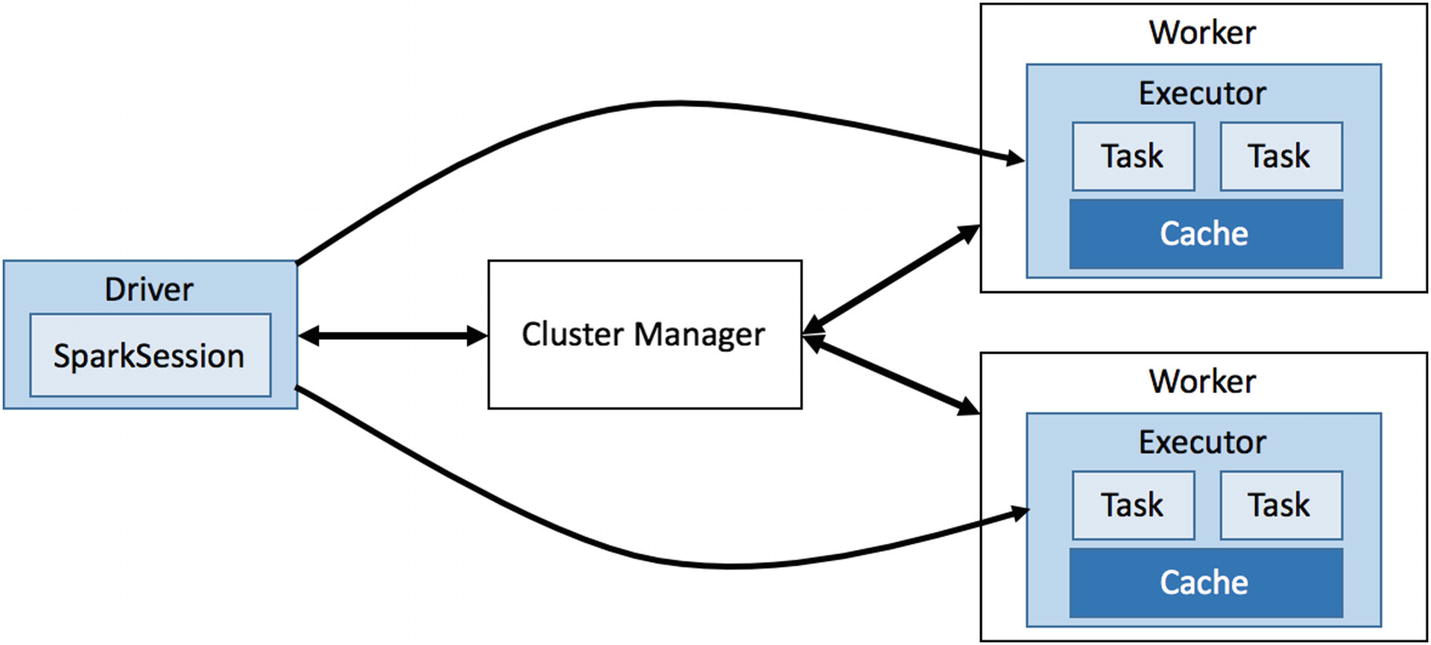
\includegraphics[width=0.7\linewidth]{illustrations/cluster-overview.jpg}
	\caption{ Interaction entre une application Spark et le cluster manager. Source : \cite{eginning-Apache-Spark-2-cluster-overwiew}}
	\label{fig:cluster-overview}
\end{figure}




\subparagraph{Application Spark} \label{sparkpresentationsection}
Une application Spark consiste en deux parties. La première partie concerne la logique décrivant les traitements à appliquer sur les données.  Cette logique est décrite en utilisant les APIs\footnote{API en Java, Scala, Python ou R.} disponibles. La deuxième partie est appelée le \textit{driver}, c'est le coordinateur principal d'une application Spark. Le driver interagit avec le cluster manager afin de trouver les machines sur lesquelles le traitement de données doit être réalisé. Ainsi, pour chacune de ces machines, le driver Spark lance le processus \textit{executor} en passant par le cluster manager. Un autre rôle du  driver Spark est de gérer et de distribuer les tâches Spark en provenance de l'application Spark sur chaque executor. Pour précision , dans la Figure \ref{fig:cluster-overview}, la classe \textit{SparkSession} est le point d'entrée vers une application Spark.

\subparagraph{Spark driver et executor}

Chaque Spark \textit{executor} est alloué exclusivement à une application Spark spécifique et la durée de vie d'un \textit{executor} est celle de l'application Spark. 

Spark utilise l'architecture master-slave. Spark \textit{driver} est le master et Spark \textit{executor} est le slave. De ce fait, une application Spark n'a qu'un seul Spark driver et plusieurs Spark \textit{executors}. Chaque Spark \textit{executor} s'occupe d'un traitement  sur une partie  des données à analyser. De cette manière,  Spark est capable de traiter  les données de façon parallèle. 
%La Figure \ref{fig:small-cluster-3} illustre un exemple d'un cluster. Ce dernier est composé de trois \textit{executors}.
%\begin{figure}[H]
%	\centering
%	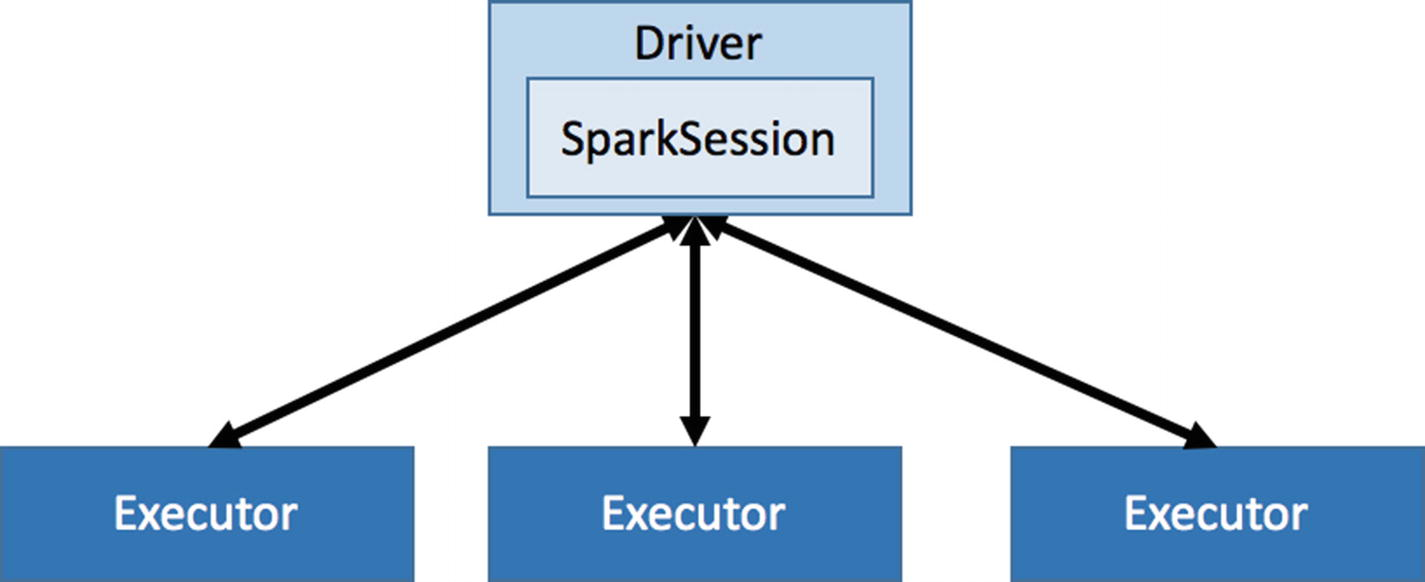
\includegraphics[width=0.7\linewidth]{illustrations/small-cluster-3}
%	\caption{Un exemple d'un cluster formé de trois executors. Source : \cite{eginning-Apache-Spark-2-cluster-example}}
%	\label{fig:small-cluster-3}
%\end{figure}


\subparagraph{Spark Unified Stack} \label{Spark Uniffied-Stack}Spark offre ce qu'on appelle Spark \textit{Stack}. C'est un ensemble de composantes construites au dessus de la composante Spark Core.  Ces composantes sont conçues pour répondre à des besoins spécifiques :
\begin{itemize}
	\item Spark SQL  est conçu effectuer des traitements sur des données structurées. Les traitements s'effectuent en se basant sur des requêtes SQL;
	\item Spark Streaming est utilisé pour les traitements    en temps réel des données en flux;
	\item  GraphX est destiné au traitement de graphes. Des fonctionnalités sont offertes afin d'analyser les graphes;
	\item MLib est conçu pour le machine learning. Ceci inclut la disponibilité des différents algorithmes et utilitaire du machine learning. Par exemple, les algorithmes de clustering, la classification, etc;
	\item SparkR est consacré aux traitements liés au machine learning en utilisant  R.
\end{itemize}
\subparagraph{Spark Core} est la base du moteur Spark pour le traitement distribué de données.  On distingue deux parties formant Spark Core. Premièrement, la partie concernant l'infrastructure distribuée du calcul. Cette dernière est responsable de la distribution, de la coordination et de la planification des tâches  sur les différentes machines formant le cluster. De plus, cette partie gère l'échec d'un traitement donné et le transfert de données entre les machines. Le deuxième élément formant Spark Core est appelé RDD (Resilient Distributed Dataset). Un RDD est une collection partitionnée d'objets, tolérante aux pannes et en lecture seule. 
%La Figure \ref{fig:unified-stack}  présente les différentes entités du Spark Unified Stack avec Spark Core.
%\begin{figure}[H]
%	\centering
%	\captionsetup{justification=centering}
%	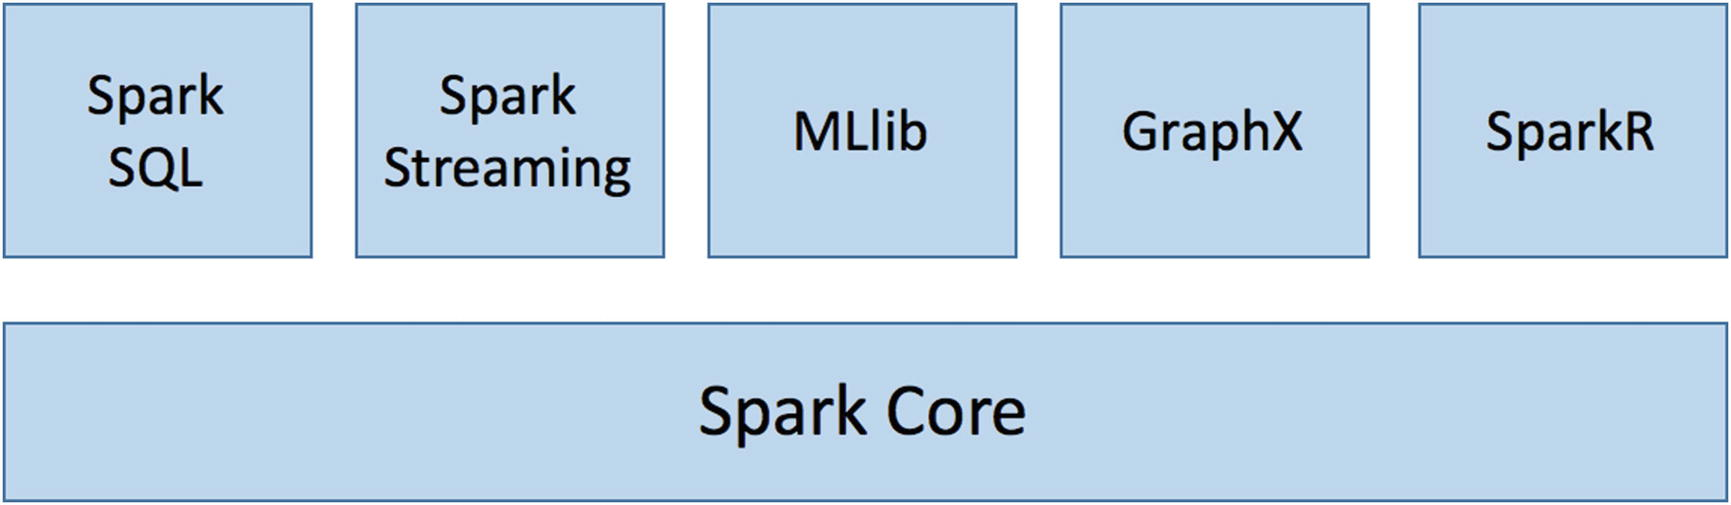
\includegraphics[width=0.7\linewidth]{illustrations/unified-stack}
%	\caption{ Spark Unified Stack. Source : \cite{eginning-Apache-Spark-2-unified-stack}}
%	\label{fig:unified-stack}
%\end{figure}

\paragraph{Resilient Distributed Datasets}\label{rdd-presentation} ~


Spark dispose d'une abstraction notée Resilient Distributed Datasets (ou RDDs). Un RDD est une collection d'objets immuable. Ces objets sont répartis sur les n\oe{}uds du cluster afin d'être traités en parallèle. Un RDD peut être conservé  pour une éventuelle réutilisation. On distingue deux manières de persistance. La conservation du RDD dans la mémoire (in-memory) ce que garantit l'amélioration des performances. En outre, un RDD peut être aussi conservé dans un disque. 

Les RDDs supportent deux types d'opérations sur les objets stockés : les transformations et les actions. Une  transformation appliquée sur un RDD crée un nouveau RDD, par exemple la transformation \textit{filter} retourne un RDD ayant vérifié la condition donnée en entrée.  Pour les actions, une action appliquée sur un RDD retourne une seule valeur, par exemple l'action \textit{count} compte le nombre d'objets d'un RDD.



%Dans la Figure 	\ref{fig:globalviewrdd}, Input data représente  les données à analyser en utilisant Spark. Ces données sont récupérées depuis des sources extérieures vers Spark. Ce dernier crée un RDD basé sur ces données. Un RDD est représenté par le rectangle en orange, les morceaux en orange dans le rectangle représentent les partitions d'un RDD. 
%On peut enchaîner plusieurs transformations sur un RDD. Comme une transformation est à la base  \textit{lazy}, les partitions ne sont partagées sur les n\oe{}uds du cluster qu'à la suite de l'appel d'une action. Une fois qu'une partition est localisée sur un n\oe{}ud donné, les transformations ainsi que les actions peuvent s'enchaîner.


 La Figure 	\ref{fig:globalviewrdd} illustre un flux de données avec l'utilisation de Spark. Dans cette figure, \textit{input data} représente les données qu'on souhaite analyser. Ces dernières sont en provenance de sources de stockage externes. Le framework Spark crée le RDD représenté par le premier rectangle orange à gauche. Ce dernier  comprend  des petits rectangles chacun représente une partition du RDD.  Les transformations  peuvent être enchaînées sur le RDD créé sans être exécutées. Les partitions seront envoyées à travers les n\oe{}ds dés que le \textit{driver} appelle une action sur ce RDD. Un n\oe{}ud est une machine avec des ressources de stockage (\textit{disk}), de calcul (\textit{CPU}), etc. Enfin, le reste des opérations peuvent s'enchaîner  sur chaque n\oe{}ud où se trouvent les données.

En cas de perte de partition pour une raison ou une autre, Spark est capable de reproduire automatiquement la partition en question. Cette fonctionnalité est assurée via le DAG (Direct Acyclic Graph). Dans ce graphe, Spark enregistre toutes les opérations appliquées sur un RDD.

\begin{figure}[h]
	\centering
	\captionsetup{justification= centering}
	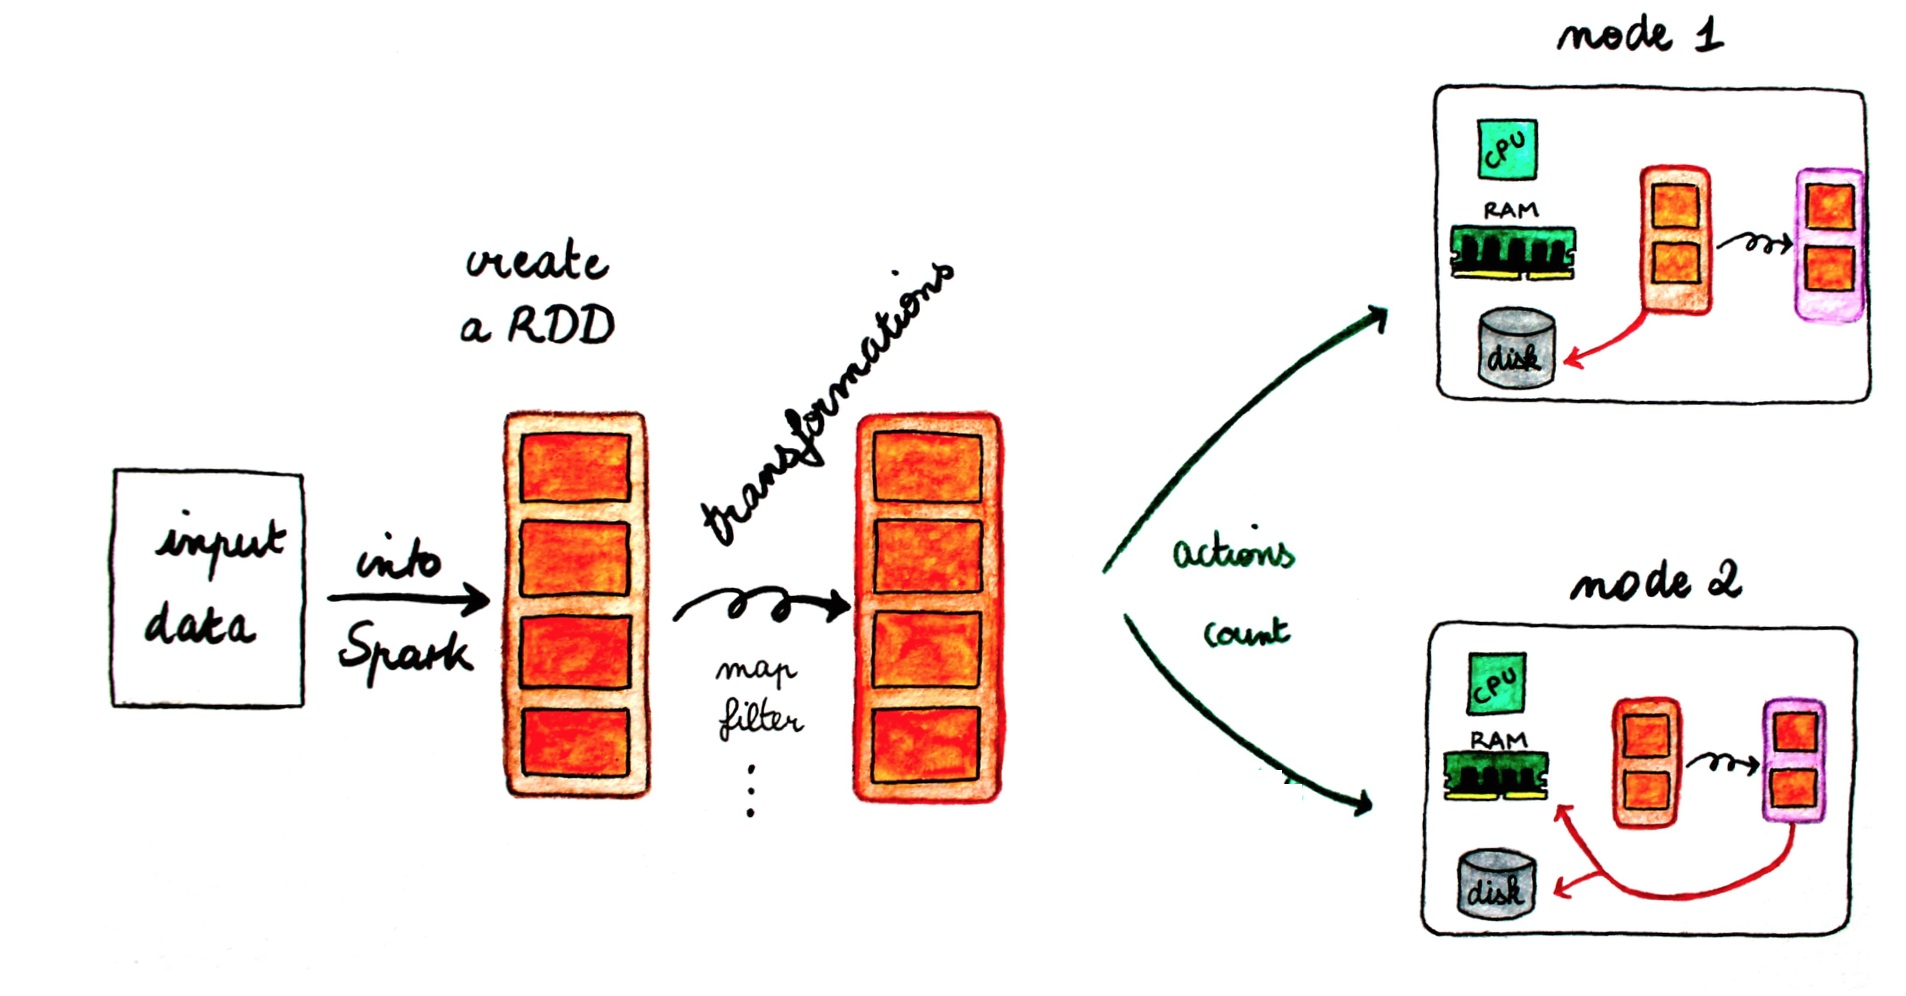
\includegraphics[width=0.7\linewidth]{illustrations/global_view_rdd}
	\caption{Exemple d'un flux de données avec Spark}
	\label{fig:globalviewrdd}
	\source{ \url{https://www.duchess-france.org/starting-with-spark-in-practice/}, consultée le $15/12/2018$.}
\end{figure}

%Resilient Distributed Dataset (RDD) allows Spark to transparently store data on the memory, and send to disk only what’s important or needed. As a result, a lot of time that is spent on the disc read and write is saved.

%Le RDD (Resilient Distributed Dataset) permet à Spark de stocker des données de manière transparente dans la mémoire et d’envoyer sur disque uniquement ce qui est important ou nécessaire. En conséquence, une grande partie du temps consacré à la lecture et à l'écriture du disque est enregistrée.[!]

\paragraph{Lazy evaluation} \label{lazy-evaluation}
Une transformation en Spark est considérée comme \textit{lazy}. Ceci implique que lorsqu'on exécute des fonctions de transformation en Spark, celles-ci ne sont pas exécutées de suite. Par contre, elles sont enregistrées dans le graphe (DAG).  Les transformations sont exécutées une fois le \textit{driver} invoque un appel à une fonction de type action. \textit{Lazy} ou l'évaluation paresseuse est un mécanisme permettant d'éviter le chargement de données depuis la source tant que ceci n'est pas nécessaire. Par conséquent, cela peut améliorer considérablement les performances.


 




%\paragraph{Les APIs de Spark}

%Le framework Spark a été écrit en Scala.  Il existe plusieurs APIs pour utiliser les fonctionnalités fournies par ce framework : Scala, Python, Java et R. 
%Il n'est pas évident de choisir entre ces quatre langages, car ce choix dépend du contexte de l'analyse. 


%Nous allons comparer ces langages dans le contexte du Big Data.



\paragraph{Les APIs du Spark}~

Spark dispose des APIs standards permettant aux développeurs  de créer une application Spark. Il existe une API en Scala, Python, Java et R. 

\paragraph{Lancement d'une application avec de Spark} \label{spark-master-modes}~

%Afin de pouvoir exécuter une application Spark, il faut l'installer. 
On distingue deux modes d'exécution d'une application  Spark : cluster et local. En  mode local, l'application  peut être exécuté au sein d'une machine locale. Par exemple,  avec un seul \textit{worker} thread (aucun parallélisme),  en précisant $K$ \textit{worker} sur $K$ threads, idéalement $K$ est le nombre des  c\oe{}urs de la machine sur laquelle Spark est installé, etc. 
 Pour le mode cluster, on distingue plusieurs types de clusters. Ces derniers  varient suivant le gestionnaire de ressources qui assure la communication entre les différentes entités du cluster selon le principe master-slave. Par exemple Hadoop YARN\footnote{URL : \url{https://hadoop.apache.org/docs/current/hadoop-yarn/hadoop-yarn-site/YARN.html}, consulté  le $14/05/2019$ } et Apache Mesos\footnote{URL : \url{https://mesos.apache.org/}, consulté le $14/05/2019$.}. La liste détaillée des alternatives pour chaque mode est donnée dans le site Web de Spark\footnote{URL : \url{https://spark.apache.org/docs/latest/submitting-applications.html\#master-urls}, consulté le $14/05/2019$.}. 
 
Il est possible d'installer Spark dans un cluster Amazon EMR (Elastic MapReduce)\footnote{URL  : \url{https://aws.amazon.com/fr/emr/}, consulté le $08/05/2019$.}. Par défaut, ce cluster utilise YARN comme gestionnaire de ressources.

\paragraph{Apache Spark VS Apache Hadoop}

Hadoop MapReduce est considéré dans \cite{Global-Journals} comme étant moins rapide en le comparant au framework Apache Spark.  Une étude \cite{article-comparaison-spark-hadoop} comparative entre Hadoop MapReduce et Spark a montré que Spark est $ 3 $ à $ 4 $ fois rapide que Hadoop MapReduce.
 Ceci est dû au fait que Spark traite les données suivant l'approche in-memory. Tandis que  les traitements basés sur le framework Hadoop sont basés sur des lectures/écritures sur le disque.  
%http://csjournals.com/IJCSC/PDF7-2/13.%20JP.pdf
\subsection{Amazon Elastic MapReduce} \label{emr-aws-presentation}

Amazon Elastic MapReduce\footnote{URL : \url{https://docs.aws.amazon.com/fr_fr/emr/}, onsulté le $10/05/2019$.} (EMR) est  un service Web proposé par Amazon  destiné aux traitements des données massives en utilisant Apache Hadoop, Apache Spark et autres.
Amazon EMR distribue le traitement de données à travers un cluster  de machines virtuelles redimensionnable. Ces machines sont des instances de type Amazon EC2\footnote{URL : \url{https://aws.amazon.com/ec2/}, consulté le $14/05/2019$.}.
Il existe plusieurs variantes d'instances EC2. Les instances sont conçues pour répondre 
aux besoins classés par AWS dans les catégories suivantes : usage général, calcul optimisé, calcul accéléré et stockage optimisé.
Elles se varient suivant leurs caractéristiques techniques comme la  RAM disponible, le nombre de CPUs, le nombre de c\oe{}urs physiques, etc. Les coûts d'utilisation des instances EC2 dépendent de ces caractéristiques,  de la région où se trouvent ces instances et du temps d'utilisation. Le coût d'utilisation des instances EC2 indépendamment d'EMR est différent du cas où une instance est utilisée pour former un cluster EMR.

Par défaut, Amazon EMR utilise YARN pour gérer les ressources. On distingue trois types de n\oe{}uds dans Amazon EMR. 
\begin{itemize}
	\item N\oe{}ud principal (\textit{Master node}) : il gère le cluster.
	\item N\oe{}ud de noyau (\textit{Core node}): exécute les tâches et stocke les données dans le système de fichier distribué Hadoop HDFS sur le cluster.
	\item N\oe{}ud de  tâche (\textit{Task node}) : il exécute les tâches et ne stocke pas les données dans HDFS. Les n\oe{}uds de tâches sont facultatifs.
\end{itemize}

Les coûts appliqués  à l'utilisation du service Amazon EMR dépendent des caractéristiques techniques des entités du cluster, la région d'Amazon choisie du cluster et enfin le temps d'utilisation du cluster. Il est possible d'estimer les frais d'utilisation d'Amazon EMR via le calculateur disponible sur le site Web d'Amazon\footnote{URL : \url{https://calculator.s3.amazonaws.com/index.html\#s=EMR}, consultée le $14/05/2019$.}.


\section{Conclusion}

Dans ce chapitre,  nous avons décrit brièvement  quelques technologies du Big Data, car la liste de toutes les technologies est très longue. Afin de découvrir ces technologies en pratique, nous allons aborder dans le chapitre \ref{chap:application-on-traceroutes} l'utilisation de ces technologies dans le cas de l'analyse des délais d'un lien décrite dans la chapitre \ref{chap:algorith-detection}.    









